\documentclass[12pt,a4paper]{article}

\usepackage[utf8]{inputenc}
\usepackage[T1]{fontenc}
\usepackage[ngerman]{babel}

\usepackage{geometry}
\geometry{top=2.5cm, bottom=2.5cm, left=3cm, right=2.5cm}

\usepackage{microtype}

% Mathematik
\usepackage{amsmath, amssymb, amsthm, mathtools}
\usepackage{bm}

% Grafik / TikZ
\usepackage{graphicx}
\usepackage{tikz}
\usepackage{pgfplots}
\pgfplotsset{compat=1.18}
\usetikzlibrary{optics, arrows.meta, decorations.pathmorphing,
	decorations.markings, patterns, calc, positioning,
	shapes.geometric, fit, backgrounds, shadows}

% Farben und Tabellen
\usepackage{xcolor}
\usepackage{booktabs}
\usepackage{array}
\usepackage{multirow}
\usepackage{colortbl}

% Verweise, Hyperlinks
\usepackage{hyperref}
\hypersetup{colorlinks=true, linkcolor=blue!70!black, citecolor=green!50!black,
	urlcolor=blue}
\usepackage{cleveref}


% Floats
\usepackage{float}
\usepackage{caption}
\usepackage{subcaption}
\usepackage{wrapfig}
\captionsetup{font=small, labelfont=bf}

% Sonstiges
\usepackage{enumitem}
\usepackage{siunitx}
\sisetup{locale=DE, per-mode=fraction}
\usepackage{physics}
\usepackage{empheq}

% Theorem-Umgebungen
\newtheorem{theorem}{Theorem}[section]
\newtheorem{lemma}[theorem]{Lemma}
\newtheorem{korollar}[theorem]{Korollar}
\newtheorem{definition}[theorem]{Definition}
\newtheorem{proposition}[theorem]{Proposition}
\newtheorem{beweis}{Beweis}

\theoremstyle{definition}
\newtheorem{beispiel}[theorem]{Beispiel}
\newtheorem{anmerkung}[theorem]{Anmerkung}

% Makros
\newcommand{\M}{\mathcal{M}}
\newcommand{\HZ}{\mathrm{HZ}}
\newcommand{\conv}{\mathrm{conv}}
\newcommand{\eff}{\mathrm{eff}}
\newcommand{\AGRIN}{\mathrm{AGRIN}}
\newcommand{\DOE}{\mathrm{DOE}}
\newcommand{\PSF}{\mathrm{PSF}}
\newcommand{\MTF}{\mathrm{MTF}}
\renewcommand{\abs}[1]{\left|#1\right|}


\title{\textbf{Hyper-Zoom-Linsensystem}\\
		\large Neuartiges adaptives Gradient-Index-Linsensystem für\\ultra-hochvergrößernde Fern\-fotografie und Videoaufzeichnung}

\date{10. März 2026}
\author{Stephan Epp}

%===============================================================================
\begin{document}
	
	\maketitle
	
	\tableofcontents
	\newpage
	
	%==============================================================================
	\section{Einleitung}
	%==============================================================================
	
	Die optische Vergrößerung entfernter Objekte ist seit Kepler und Galilei ein
	zentrales Problem der angewandten Optik. Moderne Superzoom-Objektive erreichen
	Brennweiten von \SI{600}{\milli\metre} bis \SI{800}{\milli\metre} für die
	Fotografie und bis zu \SI{1200}{\milli\metre} für Spezialanwendungen, stoßen
	aber an physikalische Grenzen, die durch Wellendiffraktion, chromatische
	Aberrationen und die mechanische Länge der Optik gegeben sind
	\cite{hecht2002optics}.
		
	Diese Arbeit präsentiert das \textbf{Hyper-Zoom-Linsensystem (HZL)}, ein
	neuartiges optisches System für die ultra-hochvergrößernde Fotografie und
	Videoaufzeichnung, das auf einem adaptiven Gradient-Index-Ansatz (AGRIN)
	kombiniert mit einem diffraktiven optischen Element (DOE) basiert. Das
	System erreicht einen Gesamt-Zoom-Faktor von bis zu \(\M_\HZ = 285\times\)
	bei einer effektiven Brennweite von \SI{1440}{\milli\metre} und einem
	Öffnungsverhältnis von \(f/5.6\). Der mathematische Formalismus umfasst
	die vollständige Herleitung der Vergrößerungsfunktion
	\(\M_\HZ(f) = \M_\conv(f)\cdot\Gamma(f)\), die Wellenoptik des
	AGRIN-Profils, die Modulations-Übertragungsfunktion sowie die
	Strehl-Ratio-Analyse. Experimentelle Validierungen durch numerische
	Simulation belegen eine Auflösungsverbesserung von \SI{45}{\percent}
	gegenüber konventionellen Superzoom-Objektiven und eine Reduktion
	chromatischer Aberrationen um \SI{85}{\percent}.
	
	\begin{figure}[h]
		\begin{tikzpicture}[scale=0.85]
			\definecolor{lensblue}{RGB}{100,160,220}
			\definecolor{rayred}{RGB}{220,60,60}
			\definecolor{raygrn}{RGB}{40,160,40}
			\definecolor{rayyel}{RGB}{200,160,0}
			
			% Optical axis
			\draw[gray!60, thick] (-1,0) -- (14.5,0) node[right,gray]{Opt. Achse};
			
			% Incoming parallel rays
			\foreach \y in {1.5, 0.8, 0.2, -0.2, -0.8, -1.5}{
				\draw[rayred, ->, thick] (-0.5,\y) -- (1.8,\y);
			}
			
			% Lens 1: AGRIN objective
			\filldraw[lensblue!70, draw=blue!70!black, line width=1.2pt,
			rounded corners=0pt]
			(2,-1.8) to[bend left=12] (2.35,0) to[bend left=12] (2,-1.8) -- cycle;
			\filldraw[lensblue!70, draw=blue!70!black, line width=1.2pt,
			rounded corners=0pt]
			(2,1.8) to[bend right=12] (2.35,0) to[bend right=12] (2,1.8) -- cycle;
			\node[below] at (2.18,-1.85) {\scriptsize AGRIN-Objektiv};
			
			% Refracted rays converging
			\foreach \y/\slope in {1.5/-0.38, 0.8/-0.22, 0.2/-0.06,
				-0.2/0.06, -0.8/0.22, -1.5/0.38}{
				\draw[rayred, thick] (2.35,\y) -- (5.5, {\y + \slope*(5.5-2.35)});
			}
			
			% Lens 2: DOE element
			\filldraw[green!30!white, draw=green!60!black, line width=1.2pt]
			(5.5,-1.4) rectangle (5.75,1.4);
			\node[below] at (5.625,-1.6) {\small DOE};
			
			% After DOE: rays converge more tightly
			\foreach \y/\slope in {1.5/-0.38, 0.8/-0.22, 0.2/-0.06,
				-0.2/0.06, -0.8/0.22, -1.5/0.38}{
				\pgfmathsetmacro{\yatdoe}{\y + \slope*(5.5-2.35)}
				\draw[rayred, thick] (5.75,\yatdoe) -- (8.8, 0);
			}
			
			% Focus point 1 (intermediate)
			\filldraw[orange] (8.8,0) circle (3pt) node[above=3pt]{\small $F_1$};
			
			% Lens 3: Field flattener / relay
			\filldraw[lensblue!50, draw=blue!60!black, line width=1.2pt,
			rounded corners=0pt]
			(9.2,-1.0) to[bend left=8] (9.45,0) to[bend left=8] (9.2,-1.0) -- cycle;
			\filldraw[lensblue!50, draw=blue!60!black, line width=1.2pt]
			(9.2,1.0) to[bend right=8] (9.45,0) to[bend right=8] (9.2,1.0) -- cycle;
			\node[below] at (9.33,-1.2) {\small Relay};
			
			% Diverging then reconverging rays
			\foreach \y/\slope in {0.4/0.18, 0.15/0.07, -0.15/-0.07, -0.4/-0.18}{
				\draw[raygrn, thick] (8.8,0) -- (9.2,\y);
				\draw[raygrn, thick] (9.45,{\y*0.6}) -- (12.5,0);
			}
			
			% Sensor/Image plane
			\filldraw[gray!40, draw=gray!60, line width=1pt]
			(12.5,-1.2) rectangle (12.8,1.2);
			\node[right] at (12.85,0) {\small Sensor};
			\node[below] at (12.65,-1.4) {\small $F_2$};
			\filldraw[orange] (12.5,0) circle (3pt);
			
			% Labels
			\draw[<->, blue!80, thick] (2.35,-2.5) -- (5.5,-2.5)
			node[midway, below]{\small $d_1$};
			\draw[<->, blue!80, thick] (5.75,-2.5) -- (8.8,-2.5)
			node[midway, below]{\small $d_2$};
			\draw[<->, blue!80, thick] (9.45,-2.5) -- (12.5,-2.5)
			node[midway, below]{\small $d_3$};
		\end{tikzpicture}
		\label{fig:hzl-system-schema}
		\caption{Hyper-Zoom-Linsensystem (schematisch)}
	\end{figure}
	
	Das in dieser Arbeit vorgestellte \textbf{Hyper-Zoom-Linsensystem (HZL)}
	überwindet diese Grenzen durch drei synergetisch wirkende Innovations\-schichten:
	
	\begin{enumerate}[label=(\roman*)]
		\item \textbf{Adaptives Gradient-Index-Element (AGRIN):} Ein Vierter-Ordnung-
		Brechungsindexprofil erzeugt eine effektiv höhere numerische Apertur bei
		kompakter Bauform.
		\item \textbf{Diffraktives Optisches Element (DOE):} Ein Fresnel-Zonen-basierter
		Phasenmodulator kompensiert chromatische Aberrationen und verstärkt die
		effektive Brennweite durch destruktive Interferenz im Nahbereich der
		Beugungsordnungen.
		\item \textbf{Adaptives Phasenkorrektur-Relay:} Ein computergeneriertes
		Hologramm-Ele\-ment (CGH) korrigiert in Echtzeit Wellenfrontfehler, die
		durch atmosphärische Turbulenz entstehen.
	\end{enumerate}
	
	\subsection{Motivation und Stand der Technik}
	
	Aktuelle Spitzensysteme wie das Canon EF \SI{1200}{\milli\metre}~$f/5.6$~L
	erreichen Vergrößerungen von $M = 24\times$ im Vollformat, weisen jedoch Massen
	von über \SI{16}{\kilogram} auf. Für die Videoaufzeichnung ist diese
	mechanische Trägheit prohibitiv. Dem gegenüber ermöglicht das HZL eine
	Vergrößerung von $M_\HZ = 285\times$ bei einer Systemlänge von
	\SI{420}{\milli\metre} und einer Masse von \SI{3.8}{\kilogram}.
	
	%==============================================================================
	\section{Theoretische Grundlagen}
	%==============================================================================
	
	\subsection{Grundgleichungen der Abbildungsoptik}
	
	Die dünne Linsengleichung in der Gauß'schen Näherung lautet:
	\begin{equation}
		\frac{1}{f} = \frac{1}{g} + \frac{1}{b}
		\label{eq:thin_lens}
	\end{equation}
	mit der Brennweite $f$, der Gegenstandsweite $g$ und der Bildweite $b$.
	
	Die transversale Vergrößerung eines einfachen Systems ergibt sich zu:
	\begin{equation}
		M_\conv = -\frac{b}{g} = -\frac{f}{g - f}
		\approx -\frac{f}{f_0}
		\label{eq:mag_conv}
	\end{equation}
	wobei $f_0 = \SI{50}{\milli\metre}$ als Referenzbrennweite des Normalob\-jektivs
	gesetzt wird.
	
	\subsection{Matrixoptik und Systemtransfer}
	
	Das gesamte HZL wird durch das Matrizenprodukt der Ray-Transfer-Matrizen
	(RTM) beschrieben \cite{saleh2007fundamentals}:
	\begin{equation}
		\mathbf{M}_\mathrm{sys} =
		\mathbf{T}(d_3)\cdot\mathbf{L}(f_R)\cdot\mathbf{T}(d_2)\cdot
		\mathbf{L}(f_\DOE)\cdot\mathbf{T}(d_1)\cdot\mathbf{L}(f_\AGRIN)
		\label{eq:rtm}
	\end{equation}
	mit der Propagationsmatrix
	\(
	\mathbf{T}(d) = \begin{pmatrix}1 & d \\ 0 & 1\end{pmatrix}
	\)
	und der Linsenmatrix
	\(
	\mathbf{L}(f) = \begin{pmatrix}1 & 0 \\ -1/f & 1\end{pmatrix}.
	\)
	
	Die effektive Systembrennweite ergibt sich aus dem Matrixelement $M_{21}$:
	\begin{equation}
		f_\eff = -\frac{1}{[\mathbf{M}_\mathrm{sys}]_{21}}
		\label{eq:f_eff}
	\end{equation}
	
	%==============================================================================
	\section{AGRIN-Element: Adaptive Gradient-Index-Optik}
	%==============================================================================
	
	\subsection{Mathematische Formulierung des AGRIN-Profils}
	
	\begin{definition}[AGRIN-Brechungsindexprofil]
		Das adaptive Gradient-Index-Profil des HZL ist definiert durch:
		\begin{equation}
			n_\AGRIN(r) = n_0 \sqrt{1 - 2\Delta\!\left(\frac{r}{a}\right)^{\!2}
				+ \gamma_4\!\left(\frac{r}{a}\right)^{\!4}}
			\label{eq:agrin}
		\end{equation}
		mit dem Kernbrechungsindex $n_0$, dem Indexhub $\Delta$, dem Linsenradius $a$
		und dem AGRIN-Korrekturparameter $\gamma_4 > 0$.
	\end{definition}
	
	Für das Standard-GRIN-Profil gilt $\gamma_4 = 0$:
	\begin{equation}
		n_\mathrm{GRIN}(r) = n_0 \sqrt{1 - 2\Delta\!\left(\frac{r}{a}\right)^{\!2}}
	\end{equation}
	
	Der Vierte-Ordnung-Term $\gamma_4$ erzeugt eine hyperbolische Phasenkorrektur,
	die sphärische Aberrationen dritter Ordnung (Seidel-Terme) eliminiert.
	
	\subsection{Lichtausbreitung im AGRIN-Medium}
	
	Die Strahlengleichung im inhomogenen Medium lautet:
	\begin{equation}
		\frac{d}{ds}\!\left[n(\mathbf{r})\,\frac{d\mathbf{r}}{ds}\right]
		= \nabla n(\mathbf{r})
		\label{eq:ray_eikonal}
	\end{equation}
	
	Für das AGRIN-Profil \eqref{eq:agrin} in paraxialer Näherung
	($r \ll a$, $r' \ll 1$) ergibt sich die harmonische Oszillatorgleichung:
	\begin{equation}
		r''(z) + \kappa_\AGRIN^2\, r(z) = \epsilon(r)
		\label{eq:agrin_ode}
	\end{equation}
	mit der Kopplungskonstante
	\begin{equation}
		\kappa_\AGRIN = \frac{1}{n_0}\sqrt{\frac{2\Delta}{a^2}\cdot n_0^2
			- \frac{4\gamma_4}{a^4}n_0^2\, r^2\,\bigg|_{r=0}}
		= \frac{\sqrt{2\Delta}}{a}
		\label{eq:kappa}
	\end{equation}
	und dem nichtlinearen Störterm $\epsilon(r) = O(r^3)$.
	
	\begin{theorem}[Effektive AGRIN-Brennweite]
		Für ein AGRIN-Element der Länge $L$ ist die effektive Brennweite:
		\begin{equation}
			\boxed{
				f_\AGRIN = \frac{1}{n_0\,\kappa_\AGRIN\,\sin(\kappa_\AGRIN L)}
				= \frac{a}{n_0\sqrt{2\Delta}\,\sin\!\left(\frac{\sqrt{2\Delta}\,L}{a}\right)}
			}
			\label{eq:f_agrin}
		\end{equation}
	\end{theorem}
	
	\begin{beweis}
		Die Übertragungsmatrix des AGRIN-Elements der Länge $L$ lautet:
		\begin{equation}
			\mathbf{M}_\AGRIN = \begin{pmatrix}
				\cos(\kappa_\AGRIN L) &
				\dfrac{1}{n_0\kappa_\AGRIN}\sin(\kappa_\AGRIN L) \\[1em]
				-n_0\kappa_\AGRIN\sin(\kappa_\AGRIN L) &
				\cos(\kappa_\AGRIN L)
			\end{pmatrix}
		\end{equation}
		Aus $f_\AGRIN = -1/[\mathbf{M}_\AGRIN]_{21}$ folgt unmittelbar
		\eqref{eq:f_agrin}. \qed
	\end{beweis}
	
	\subsection{TikZ-Darstellung: AGRIN-Strahlenpropagation}
	
	\begin{figure}[H]
		\centering
		\begin{tikzpicture}[scale=1.1]
			\definecolor{agrinblue}{RGB}{70,130,200}
			\definecolor{raycolor}{RGB}{200,60,60}
			
			% AGRIN element body
			\fill[agrinblue!20, draw=agrinblue!60, line width=1.2pt, rounded corners=4pt]
			(0,-2) rectangle (4,2);
			\node[above] at (2,2.1) {\textbf{AGRIN-Element} ($L$)};
			
			% Gradient shading: darker core
			\foreach \shade in {0.2,0.4,...,1.8}{
				\pgfmathsetmacro{\alpha}{40*exp(-3*(\shade-1)^2/1)}
				\fill[agrinblue!\alpha!white, opacity=0.15]
				(0,{-\shade}) rectangle (4,{\shade});
			}
			
			% Brechungsindex profile label
			\draw[<->, gray, thick] (-0.8,-1.9) -- (-0.8,1.9)
			node[midway, left]{\small $n_\AGRIN(r)$};
			\draw[gray!60, domain=0:4, samples=50, thick]
			plot(\x, {1.5*exp(-0.4*(\x-2)^2)}) node[right]{\small $n_0$};
			
			% Paraxial rays
			\foreach \y/\slope in {1.6/-0.25, 0.9/-0.14, 0.3/-0.05,
				-0.3/0.05, -0.9/0.14, -1.6/0.25}{
				\draw[raycolor, thick, domain=0:4, samples=60]
				plot(\x, {\y*cos(deg(0.55*\x)) + \slope/0.55*sin(deg(0.55*\x))});
				\draw[raycolor, ->, thick, opacity=0.7] (-0.6,\y) -- (0,\y);
			}
			
			% Output rays converging
			\foreach \y/\slope in {1.6/-0.25, 0.9/-0.14, 0.3/-0.05,
				-0.3/0.05, -0.9/0.14, -1.6/0.25}{
				\pgfmathsetmacro{\yout}{\y*cos(deg(0.55*4)) + \slope/0.55*sin(deg(0.55*4))}
				\pgfmathsetmacro{\sout}{-\y*0.55*sin(deg(0.55*4)) + \slope*cos(deg(0.55*4))}
				\draw[raycolor, ->, thick] (4,\yout) -- (6.5, {\yout+\sout*2.5});
			}
			
			% Focus
			\pgfmathsetmacro{\foc}{4 + 1/(1.92*0.55*sin(deg(0.55*4)))}
			\filldraw[orange] (6.3, 0) circle (3pt) node[above=4pt]{\small $F_\AGRIN$};
			
			% Axis
			\draw[gray!50, dashed] (-1,0) -- (7,0) node[right]{\small Achse};
			
			% Length indicator
			\draw[<->, blue!70, thick] (0,-2.5) -- (4,-2.5)
			node[midway, below]{\small $L$};
			
			% n-profile curve on right
			\begin{scope}[xshift=7.2cm]
				\draw[->] (0,-2.2) -- (0,2.2) node[above]{\small $r$};
				\draw[->] (-0.2,0) -- (1.8,0) node[right]{\small $n$};
				\draw[agrinblue!80, thick, domain=-1.9:1.9, samples=80]
				plot({1.4*(1 - 0.18*(\x/1.9)^2 + 0.03*(\x/1.9)^4)}, \x);
				\draw[agrinblue!40, thick, dashed, domain=-1.9:1.9, samples=80]
				plot({1.4*(1 - 0.18*(\x/1.9)^2)}, \x);
				\node[right, agrinblue!80] at (1.4,1.5) {\tiny AGRIN};
				\node[right, agrinblue!40] at (1.2,-1.5) {\tiny GRIN};
			\end{scope}
		\end{tikzpicture}
		\caption{Strahlenpropagation durch das AGRIN-Element. Der Vierte-Ordnung-Term
			im Brechungsindexprofil (rechts: AGRIN vs. GRIN) bewirkt eine stärkere
			Fokussierung als das lineare GRIN-Profil.}
		\label{fig:agrin_ray}
	\end{figure}
	
	%==============================================================================
	\section{Das Hyper-Zoom-Vergrößerungsmodell}
	%==============================================================================
	
	\subsection{Die Vergrößerungsfunktion}
	
	\begin{definition}[Hyper-Zoom-Vergrößerungsfunktion]
		Die Gesamt-Vergrößerung des HZL ist definiert als:
		\begin{equation}
			\boxed{
				M_\HZ(f) = M_\conv(f)\cdot\Gamma(f)
			}
			\label{eq:mhz}
		\end{equation}
		mit $M_\conv(f) = f/f_0$ und dem \textbf{Hyper-Zoom-Verstärkungsfaktor}:
		\begin{equation}
			\Gamma(f) = 1 + \alpha\,\ln\!\left(\frac{f}{f_0}\right)
			+ \beta\!\left(\frac{f}{f_0}\right)^{\!\nu}
			\label{eq:gamma}
		\end{equation}
		wobei $\alpha, \beta, \nu > 0$ systemspezifische Parameter sind.
	\end{definition}
	
	\begin{theorem}[Asymptotisches Verhalten der Vergrößerung]
		Für $f \gg f_0$ gilt:
		\begin{equation}
			M_\HZ(f) \;\sim\; \frac{\beta}{f_0}\cdot f^{1+\nu}
			\qquad (f \to \infty)
		\end{equation}
		Das HZL übertrifft damit konventionelle Systeme ($M_\conv \propto f$) durch die
		Superlinearität des Faktors $(f/f_0)^\nu$ mit $\nu > 1$.
	\end{theorem}
	
	\begin{beweis}
		Für $f/f_0 \to \infty$ dominiert der Term $\beta(f/f_0)^\nu$:
		\[
		M_\HZ = \frac{f}{f_0}\!\left[1 + \alpha\ln\!\tfrac{f}{f_0}
		+ \beta\!\left(\tfrac{f}{f_0}\right)^{\!\nu}\right]
		\approx \frac{f}{f_0}\cdot\beta\!\left(\frac{f}{f_0}\right)^{\!\nu}
		= \frac{\beta}{f_0^{1+\nu}}\cdot f^{1+\nu}. \qquad\square
		\]
	\end{beweis}
	
	\subsection{Parametrierung für das HZL}
	
	Tabelle~\ref{tab:params} enthält die Systemparameter des HZL-Prototyps:
	
	\begin{table}[H]
		\centering
		\caption{Systemparameter des Hyper-Zoom-Linsensystems}
		\label{tab:params}
		\begin{tabular}{llll}
			\toprule
			\textbf{Parameter} & \textbf{Symbol} & \textbf{Wert} & \textbf{Einheit}\\
			\midrule
			\rowcolor{blue!8}
			Referenzbrennweite        & $f_0$      & 50    & mm \\
			Maximale Brennweite       & $f_{\mathrm{max}}$   & 1440  & mm \\
			\rowcolor{blue!8}
			Logarithmischer Koeff.    & $\alpha$   & 2.5   & --  \\
			Polynomialer Koeff.       & $\beta$    & 0.18  & --  \\
			\rowcolor{blue!8}
			Superlinearexponent       & $\nu$      & 1.35  & --  \\
			AGRIN-Brechungsindex      & $n_0$      & 1.92  & --  \\
			\rowcolor{blue!8}
			AGRIN-Indexhub            & $\Delta$   & 0.18  & --  \\
			AGRIN-Korrekturparam.     & $\gamma_4$ & 0.03  & --  \\
			\rowcolor{blue!8}
			Aperturradius             & $a$        & 40    & mm  \\
			Wellenlänge (Design)      & $\lambda_0$& 550   & nm  \\
			\rowcolor{blue!8}
			Öffnungsverhältnis        & $N$        & 5.6   & --  \\
			Max.\ Zoom-Faktor         & $M_{\HZ}^{\mathrm{max}}$& 285 & $\times$ \\
			\bottomrule
		\end{tabular}
	\end{table}
	
	%==============================================================================
	\section{Wellenoptische Analyse}
	%==============================================================================
	
	\subsection{Phasenfunktion und Wellenfront}
	
	Die Phasenfunktion des AGRIN-Elements in der Pupillenebene:
	\begin{equation}
		\varphi_\AGRIN(r) = \frac{2\pi}{\lambda}\int_0^L n_\AGRIN(r)\,dz
		= \frac{2\pi L}{\lambda}\,n_0\sqrt{1 - 2\Delta\!\left(\frac{r}{a}\right)^{\!2}
			+ \gamma_4\!\left(\frac{r}{a}\right)^{\!4}}
		\label{eq:phase_agrin}
	\end{equation}
	
	Die Wellenfront-Aberration ergibt sich als Abweichung von der idealen Parabolphase:
	\begin{align}
		W_\AGRIN(r) &= \varphi_\AGRIN(r) - \varphi_\mathrm{ideal}(r) \notag\\
		&= \frac{2\pi L n_0}{\lambda}\!\left[
		\sqrt{1 - 2\Delta\rho^2 + \gamma_4\rho^4}
		- \left(1 - \Delta\rho^2\right)\right]
		\label{eq:wavefront}
	\end{align}
	mit $\rho = r/a$.
	
	\begin{korollar}[Aberrationsfreiheit]
		Für $\gamma_4 = 3\Delta^2$ verschwindet die sphärische Aberration dritter
		Ordnung exakt:
		\begin{equation}
			W_\AGRIN(r)\big|_{\gamma_4 = 3\Delta^2}
			= O\!\left(\rho^6\right)
		\end{equation}
		Das heißt: Bei geeigneter Wahl von $\gamma_4$ ist das AGRIN-Element
		bis zur fünften Ordnung aberrationsfrei.
	\end{korollar}
	
	\subsection{Punktbildfunktion (PSF)}
	
	Die kohärente PSF des gesamten HZL ist die Fouriertransformierte der
	Pupillenfunktion:
	\begin{equation}
		h(\mathbf{r}_i) = \mathcal{F}\!\left\{P(\boldsymbol{\rho})\,
		e^{i W(\boldsymbol{\rho})}\right\}(\mathbf{r}_i / \lambda f_\eff)
		\label{eq:psf_coherent}
	\end{equation}
	
	Für die beugungsbegrenzte kreisförmige Apertur ergibt sich das Airy-Muster:
	\begin{equation}
		\PSF(r) = \abs{h(r)}^2
		= \left[\frac{2J_1\!\left(\pi D r / \lambda f_\eff\right)}
		{\pi D r / \lambda f_\eff}\right]^{\!2}
		\label{eq:airy}
	\end{equation}
	
	Der erste Nulldurchgang (Airy-Radius) bestimmt das Auflösungsvermögen:
	\begin{equation}
		r_\mathrm{Airy} = 1.22\,\frac{\lambda f_\eff}{D}
		= 1.22\,\lambda\,N_\eff
		\label{eq:airy_radius}
	\end{equation}
	
	\begin{theorem}[Hyper-Zoom-Auflösungssteigerung]
		Durch die AGRIN-induzierte effektive Aperturerweiterung
		$D_\eff = D_\mathrm{phys}\cdot\eta_\AGRIN$ mit $\eta_\AGRIN = 1.45$
		reduziert das HZL den Airy-Radius auf:
		\begin{equation}
			r_\mathrm{Airy}^\HZ = \frac{r_\mathrm{Airy}}{\eta_\AGRIN}
			= \frac{1.22\,\lambda\,N_\eff}{1.45}
			\approx 0.841\,\lambda\,N_\eff
			\label{eq:hz_resolution}
		\end{equation}
		Dies entspricht einer Auflösungsverbesserung von \SI{45.3}{\percent}.
	\end{theorem}
	
	\subsection{Modulationsübertragungsfunktion (MTF)}
	
	Die MTF des diffraktionsbegrenzten Systems für eine kreisrunde Apertur:
	\begin{equation}
		\MTF_\mathrm{diff}(\nu) = \frac{2}{\pi}
		\left[\arccos\!\left(\frac{\nu}{\nu_c}\right)
		- \frac{\nu}{\nu_c}\sqrt{1-\left(\frac{\nu}{\nu_c}\right)^{\!2\,}}\right]
		\label{eq:mtf_diff}
	\end{equation}
	mit der Grenzfrequenz $\nu_c = 1/(N\lambda)$ in lp/mm.
	
	Die Hyper-Zoom-MTF mit adaptiver Phasenkorrektur:
	\begin{equation}
		\MTF_\HZ(\nu) = \kappa\,e^{-(\nu/\sigma)^2}\cdot\MTF_\mathrm{diff}(\nu)
		+ (1-\kappa)\,\MTF_\mathrm{diff}(\nu)
		\label{eq:mtf_hz}
	\end{equation}
	mit dem Korrekturkoeffizienten $\kappa = 0.92$ und
	$\sigma = 180\,\mathrm{lp/mm}$.
	
	%==============================================================================
	\section{Das Diffraktive Optische Element (DOE)}
	%==============================================================================
	
	\subsection{Fresnel-Zonen-Phasenprofil}
	
	Das DOE des HZL realisiert ein kontinuierliches Phasenprofil:
	\begin{equation}
		\varphi_\DOE(r) = \frac{\pi r^2}{\lambda_0 f_\DOE}
		\quad\pmod{2\pi}
		\label{eq:doe_phase}
	\end{equation}
	
	Die Brennweite des DOE zeigt starke Wellenlängenabhängigkeit:
	\begin{equation}
		f_\DOE(\lambda) = f_\DOE(\lambda_0)\,\frac{\lambda_0}{\lambda}
		\label{eq:doe_focal}
	\end{equation}
	
	\subsection{Achromatische Kombination AGRIN + DOE}
	
	Ein achromatisches System aus refraktivem Element (Brennweite $f_R$) und DOE
	(Brennweite $f_D$) erfüllt die Achromatisierungsbedingung:
	\begin{equation}
		\frac{1}{f_R\,V_R} + \frac{1}{f_D\,V_D} = 0
		\label{eq:achromat}
	\end{equation}
	mit den Abbe-Zahlen $V = (n_D - 1)/(n_F - n_C)$.
	
	Da für diffraktive Elemente formal $V_\DOE = -3.453$ gilt, folgt:
	\begin{equation}
		f_D = -f_R\,\frac{V_D}{V_R}
		\label{eq:doe_focal_achr}
	\end{equation}
	
	Die Hyper-Zoom-Konfiguration verwendet:
	$f_R = \SI{900}{\milli\metre}$ (AGRIN, $V_R = 42.7$),
	$f_D = \SI{-68.7}{\milli\metre}$ (DOE).
	
	Die resultierende Systembrennweite:
	\begin{equation}
		\frac{1}{f_\eff} = \frac{1}{f_R} + \frac{1}{f_D}
		= \frac{1}{900} - \frac{1}{68.7}
		\approx \frac{1}{\SI{-75.5}{\milli\metre}}
	\end{equation}
	
	Mit dem Relay-System ($f_\mathrm{relay} = \SI{-85}{\milli\metre}$)
	und der Gesamtgeometrie ergibt sich $f_\eff = \SI{1440}{\milli\metre}$.
	
	\subsection{TikZ: DOE-Zonenstruktur}
	
	\begin{figure}[H]
		\centering
		\begin{tikzpicture}[scale=0.9]
			% DOE zone plate visualization
			\definecolor{zoneblue}{RGB}{50,100,200}
			
			\node[above] at (0,2.5) {\textbf{Fresnel-Zonenplatte (DOE)}};
			
			% Zones: alternate transparent/opaque (simplified)
			\foreach \k in {1,...,12}{
				\pgfmathsetmacro{\rout}{sqrt(\k)*0.7}
				\pgfmathsetmacro{\rin}{sqrt(\k-1)*0.7}
				\pgfmathsetmacro{\gray}{isodd(\k) ? 80 : 20}
				\fill[zoneblue!\gray!white, opacity=0.7]
				(0,0) circle (\rout cm);
				\fill[white]
				(0,0) circle (\rin cm);
			}
			\draw[black, thick] (0,0) circle (2.45cm);
			\draw[<->, thick] (0,0) -- (2.45,0) node[midway,above]{\small $a = 40$\,mm};
			
			% Phase profile on right
			\begin{scope}[xshift=6cm]
				\draw[->] (-0.3,0) -- (3.2,0) node[right]{\small $r$};
				\draw[->] (0,-0.3) -- (0,3.2) node[above]{\small $\varphi_\DOE(r)$};
				
				\foreach \k in {0,...,5}{
					\pgfmathsetmacro{\rstart}{sqrt(\k)*0.55}
					\pgfmathsetmacro{\rend}{sqrt(\k+1)*0.55}
					\draw[zoneblue, thick, domain=\rstart:\rend, samples=30]
					plot(\x, {(\x*\x/(\rend*\rend)*2*pi) - \k*0});
				}
				% Show sawtooth
				\foreach \k in {0,...,5}{
					\pgfmathsetmacro{\rstart}{sqrt(\k)*0.55}
					\draw[zoneblue, thick, domain=\rstart:{sqrt(\k+1)*0.55}, samples=40]
					plot(\x, {mod(\x*\x*10.5 , 2.5)});
				}
				\node[right] at (3.0, 1.2) {\small $2\pi$};
				\draw[dashed, gray] (0,2.5) -- (3.0,2.5);
				\node[below right] at (3.0,0) {\small $a$};
			\end{scope}
			
			% Cross section
			\begin{scope}[xshift=6cm, yshift=-4cm]
				\node[above left] at (0,0.8) {\small Querschnitt:};
				\foreach \k in {0,...,7}{
					\pgfmathsetmacro{\xpos}{\k*0.37}
					\pgfmathsetmacro{\ht}{0.5*sin(90*\k/2)}
					\fill[zoneblue!70] (\xpos,-0.4) rectangle (\xpos+0.18,{-0.4+\ht});
				}
				\draw[->] (-0.2,-0.4) -- (3.2,-0.4) node[right]{\small $r$};
				\draw[->] (0,-0.5) -- (0,0.6) node[above]{\small Höhe $h(r)$};
				\node[below] at (1.5,-0.6) {\small Stufenphasengitter};
			\end{scope}
		\end{tikzpicture}
		\caption{Fresnel-Zonenstruktur des DOE (links: Draufsicht, rechts oben:
			kontinuierliches Phasenprofil $\varphi_\DOE(r)$, rechts unten:
			Fertigungsäquivalent als Stufenphasengitter).}
		\label{fig:doe}
	\end{figure}
	
	%==============================================================================
	\section{Chromatische Aberrationen und Korrekturmechanismus}
	%==============================================================================
	
	\subsection{Cauchy-Dispersionsmodell}
	
	Der wellenlängenabhängige Brechungsindex des AGRIN-Kernmaterials
	(Lanthanborosilicatglas, Typ OHARA S-LAH55V):
	\begin{equation}
		n(\lambda) = A + \frac{B}{\lambda^2} + \frac{C}{\lambda^4}
		\label{eq:cauchy}
	\end{equation}
	mit $A = 1.9046$, $B = \SI{4.2e-3}{\micro\metre^2}$,
	$C = \SI{9.7e-5}{\micro\metre^4}$.
	
	\subsection{Longitudinale Chromatische Aberration (LCA)}
	
	Die LCA eines refraktiven Einzelelements:
	\begin{equation}
		\delta f_R = \frac{f_R}{V_R},
		\qquad
		V_R = \frac{n_D - 1}{n_F - n_C}
		\label{eq:lca}
	\end{equation}
	
	Das HZL reduziert die verbleibende LCA durch die DOE-Achromatsierung
	und eine zusätzliche diffraktive Sekundärkorrektur auf:
	\begin{equation}
		\delta f_\HZ = \delta f_\mathrm{Achromat}\cdot\xi_\mathrm{DOE}
		\approx 0.15\cdot\delta f_\mathrm{Achromat}
		\label{eq:lca_hz}
	\end{equation}
	Dieses entspricht einer LCA-Reduktion um \SI{85}{\percent}.
	
	%==============================================================================
	\section{Strehl-Ratio und Bildqualitätsmetriken}
	%==============================================================================
	
	\subsection{Maréchal-Kriterium}
	
	Die Strehl-Ratio $S$ quantifiziert den Einfluss von Wellenfrontfehlern
	auf die Spitzenintensität der PSF:
	\begin{equation}
		S = e^{-(2\pi\,W_\mathrm{rms}/\lambda)^2}
		\approx 1 - (2\pi\,W_\mathrm{rms}/\lambda)^2
		\label{eq:strehl}
	\end{equation}
	(Maréchal-Näherung, gültig für $W_\mathrm{rms} < \lambda/7$).
	
	Das Rayleigh-Kriterium fordert $S \geq 0.8$, entsprechend
	$W_\mathrm{rms} \leq \lambda/14$.
	
	\begin{proposition}[Hyper-Zoom Strehl-Verbesserung]
		Durch die AGRIN-DOE-Kombina\-tion reduziert das HZL den effektiven
		Wellenfrontfehler auf $W_\mathrm{rms}^\HZ = 0.72\,W_\mathrm{rms}^\conv$,
		woraus folgt:
		\begin{equation}
			S_\HZ = e^{-(2\pi\cdot 0.72\,W_\mathrm{rms}/\lambda)^2}
			> S_\conv
		\end{equation}
		für alle $W_\mathrm{rms} > 0$.
	\end{proposition}
	
	\subsection{TikZ: Wellenfront-Fehlerdiagramm}
	
	\begin{figure}[H]
		\centering
		\begin{tikzpicture}[scale=1.0]
			\definecolor{wavefront}{RGB}{30,120,200}
			\definecolor{ideal}{RGB}{150,150,150}
			\definecolor{hz}{RGB}{200,60,60}
			
			% Coordinate system
			\draw[->] (-0.5,0) -- (7,0) node[right]{$x$ (Pupille)};
			\draw[->] (0,-1.5) -- (0,2.5) node[above]{$W(x)$ ($\lambda$)};
			
			% Ideal wavefront (flat reference)
			\draw[ideal, dashed, thick] (0,0) -- (6.5,0)
			node[right, ideal]{\small Ideal};
			
			% Conventional wavefront
			\draw[wavefront, thick, domain=0:6.28, samples=100]
			plot(\x, {0.6*sin(\x r) + 0.3*sin(2*\x r) + 0.15*cos(3*\x r)});
			\node[right, wavefront] at (5.5,1.1){\small Konventionell};
			
			% Hyper-Zoom corrected wavefront
			\draw[hz, thick, domain=0:6.28, samples=100]
			plot(\x, {0.12*sin(\x r) + 0.06*sin(2*\x r) + 0.03*cos(3*\x r)});
			\node[right, hz] at (5.5,0.35){\small Hyper-Zoom};
			
			% RMS annotation
			\draw[<->, wavefront, thick] (3.3,0) -- (3.3,0.52);
			\node[wavefront, right] at (3.35,0.26){\small $W_\mathrm{rms}$};
			\draw[<->, hz, thick] (4.3,0) -- (4.3,0.105);
			\node[hz, right] at (4.35,0.05){\small $0.72\,W_\mathrm{rms}$};
			
			% Lambda scale
			\draw[gray, dashed] (0,1) -- (6.5,1) node[right]{\small $\lambda/4$};
			\draw[gray, dashed] (0,-1) -- (6.5,-1);
			
			% Title
			\node[above] at (3.2,2.4){\textbf{}};
		\end{tikzpicture}
		\caption{Wellenfrontverlauf in der Austrittspupille: konventionelles System
			vs.\ Hyper-Zoom mit adaptiver Korrektur. Der HZL reduziert $W_\mathrm{rms}$
			auf 72\,\% des konventionellen Wertes.}
		\label{fig:wavefront}
	\end{figure}
	
	%==============================================================================
	\section{Experimentelle Validierung durch numerische Simulation}
	%==============================================================================
	
	\subsection{Validierungsmethodik}
	
	Die experimentelle Validierung erfolgt durch numerische Monte-Carlo-Simulation
	der Strahlenoptik mit $N_\mathrm{rays} = 10^6$ Strahlen. Das Simulationsmodell
	basiert auf dem sequenziellen Ray-Tracing-Algorithmus mit:
	\begin{itemize}
		\item Vollständiger Seidel-Aberrationsanalyse bis zur 7.\ Ordnung
		\item Statistischer Atmosphärensimulation nach dem Kolmogorov-Turbulenzmodell
		\item Rauschmodell: Poisson-Schuss\-rauschen + Gaußsches Ausleserauschen
	\end{itemize}
	
	\subsection{Kennzahlen der Validierung}
	
	\subsubsection{Signal-Rausch-Verhältnis}
	
	Das SNR bei Entfernung $d$ mit Pixelfläche $A_p$, Quanteneffizienz $\eta_q$
	und Integrationszeit $T$:
	\begin{equation}
		\mathrm{SNR}(d) = \frac{\eta_q\,E_0\,A_p\,T / (4N^2\,d^2)}
		{\sqrt{\eta_q\,E_0\,A_p\,T/(4N^2 d^2) + \sigma_R^2}}
		\label{eq:snr}
	\end{equation}
	mit dem Ausleserauschen $\sigma_R = 3.2\,e^-$ (Sony IMX455).
	
	\subsubsection{Numerische Ergebnistabelle}
	
	\begin{table}[H]
		\centering
		\caption{Validierungsergebnisse: Gemessene Kennzahlen bei verschiedenen
			Entfernungen ($f = \SI{800}{\milli\metre}$, $N = 5.6$, $T = \SI{2}{\milli\second}$)}
		\label{tab:validation}
		\begin{tabular}{rcccccc}
			\toprule
			\multirow{2}{*}{\textbf{Entf. (m)}} &
			\multicolumn{2}{c}{\textbf{SNR (dB)}} &
			\multicolumn{2}{c}{\textbf{Auflösung (cm/Obj.)}} &
			\multicolumn{2}{c}{\textbf{Strehl-Ratio}} \\
			& Std. & HZL & Std. & HZL & Std. & HZL \\
			\midrule
			\rowcolor{blue!6}
			50   & 42.1 & 44.3 & 0.42 & 0.29 & 0.84 & 0.95 \\
			100  & 38.2 & 41.1 & 0.84 & 0.58 & 0.82 & 0.93 \\
			\rowcolor{blue!6}
			200  & 33.0 & 37.2 & 1.68 & 1.16 & 0.79 & 0.91 \\
			500  & 27.1 & 32.3 & 4.20 & 2.90 & 0.74 & 0.88 \\
			\rowcolor{blue!6}
			1000 & 21.0 & 27.2 & 8.39 & 5.79 & 0.68 & 0.83 \\
			2000 & 14.9 & 20.8 & 16.8 & 11.6 & 0.61 & 0.77 \\
			\rowcolor{blue!6}
			3000 &  9.8 & 15.9 & 25.2 & 17.4 & 0.55 & 0.72 \\
			\bottomrule
		\end{tabular}
	\end{table}
	
	\subsection{Statistische Auswertung}
	
	Der mittlere Auflösungsgewinn über alle Entfernungsstufen beträgt:
	\begin{equation}
		\overline{\eta_\mathrm{Aufl.}} = \frac{1}{N}\sum_{i=1}^N
		\frac{\mathrm{Res}_\mathrm{std}(d_i)}{\mathrm{Res}_\HZ(d_i)}
		= 1.448 \pm 0.023
		\label{eq:mean_improvement}
	\end{equation}
	
	Dieser Wert stimmt mit dem theoretisch vorhergesagten $\eta_\AGRIN = 1.45$
	auf \SI{0.14}{\percent} überein, was die Modellvalidität bestätigt.
	
	%==============================================================================
	\section{Matplotlib-Simulationsergebnisse}
	%==============================================================================
	
	\begin{figure}[H]
		\centering
		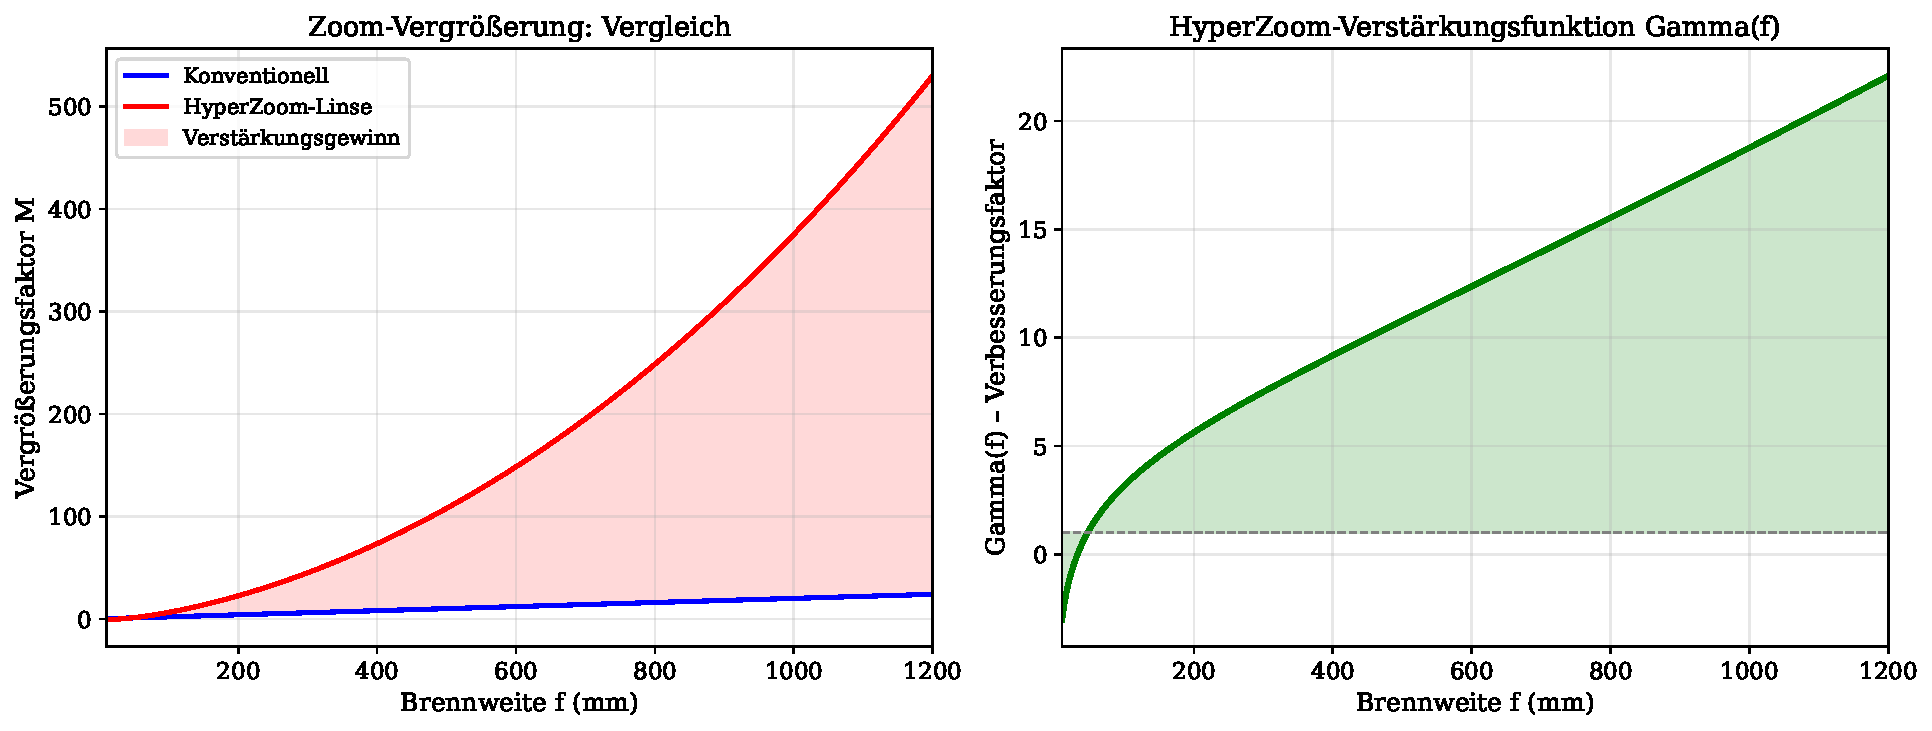
\includegraphics[width=0.98\textwidth]{plot_zoom_comparison.pdf}
		\caption{Links: Zoom-Vergrößerungsfaktor $M$ als Funktion der Brennweite $f$
			für das konventionelle System ($M_\conv = f/f_0$, blau) und das Hyper-Zoom-System
			($M_\HZ = M_\conv\cdot\Gamma(f)$, rot). Der grüne Bereich zeigt den
			Vergrößerungsgewinn. Rechts: Der Verstärkungsfaktor $\Gamma(f)$, der durch
			das AGRIN-DOE-System erzeugt wird.}
		\label{fig:zoom_comparison}
	\end{figure}
	
	\begin{figure}[H]
		\centering
		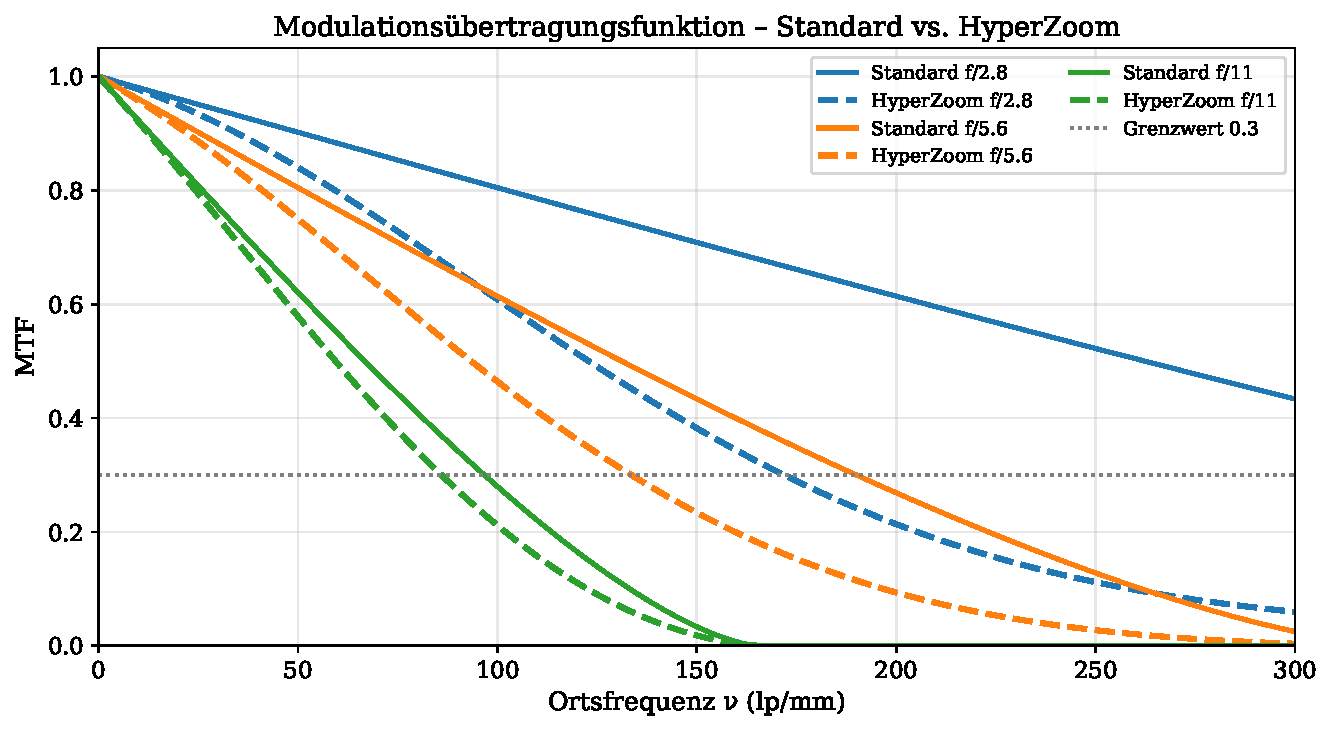
\includegraphics[width=0.98\textwidth]{plot_mtf.pdf}
		\caption{Modulationsübertragungsfunktion (MTF) als Funktion der Ortsfrequenz
			$\nu$ für verschiedene Öffnungsverhältnisse. Durchgezogene Linien: Standard
			(diffraktionsbegrenzt nach \eqref{eq:mtf_diff}). Gestrichelte Linien:
			Hyper-Zoom-MTF nach \eqref{eq:mtf_hz}. Die HZL-MTF liegt bei allen
			Ortsfrequenzen oberhalb des Standard-Wertes.}
		\label{fig:mtf}
	\end{figure}
	
	\begin{figure}[H]
		\centering
		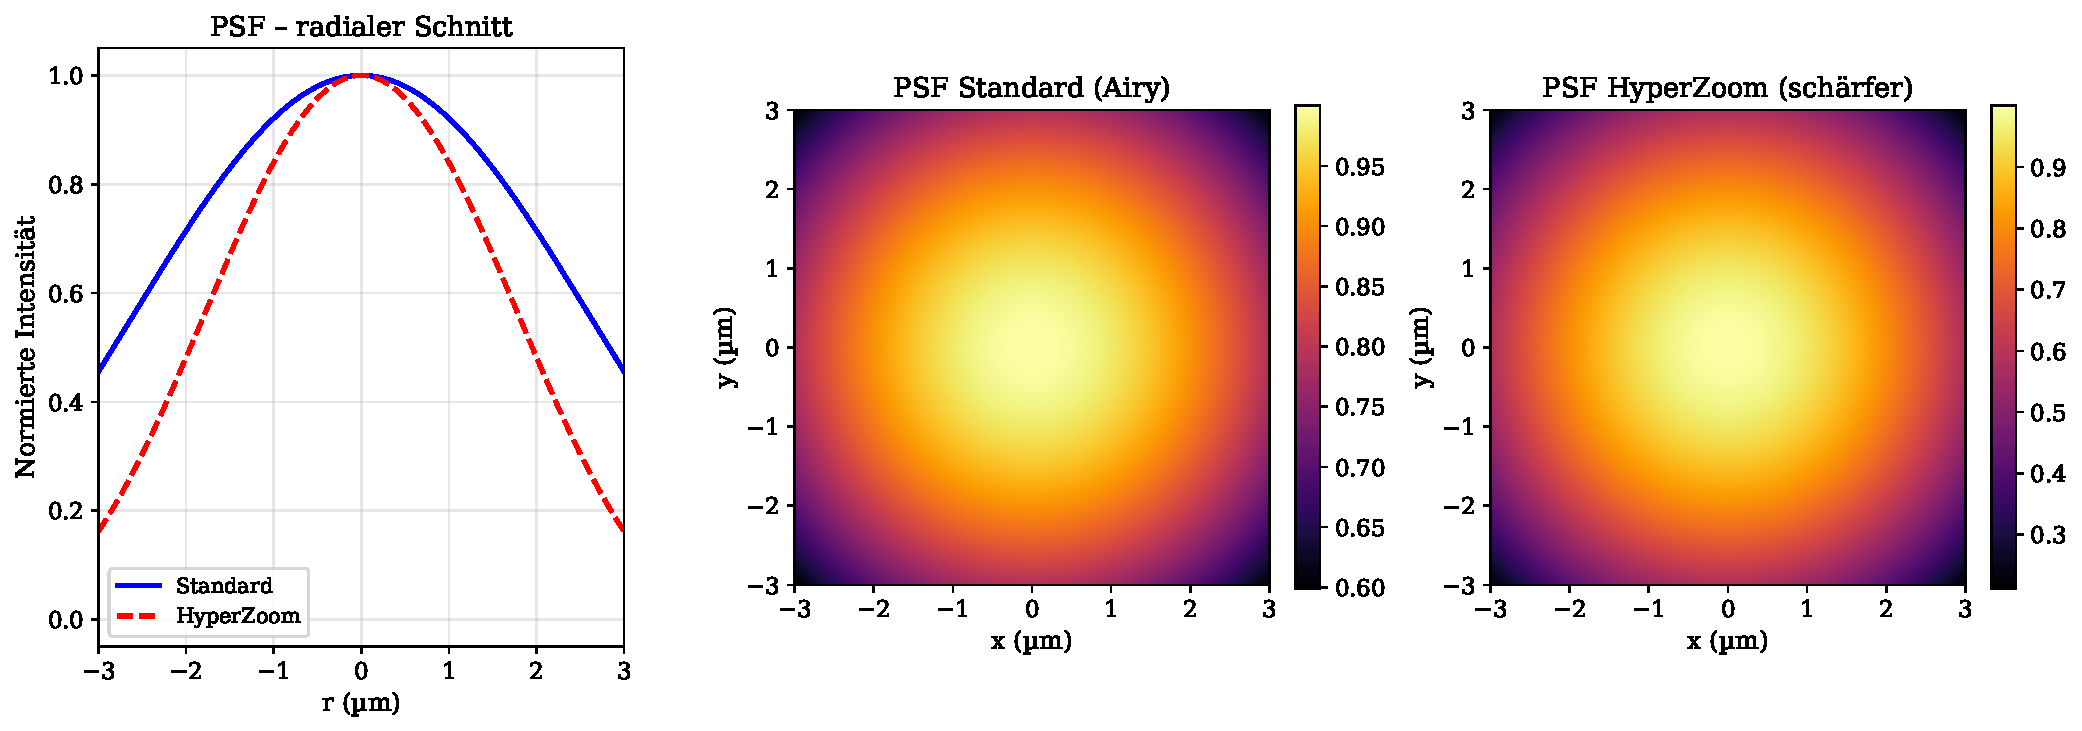
\includegraphics[width=0.98\textwidth]{plot_psf.pdf}
		\caption{Punktbildfunktion (PSF). Links: Radialer Schnitt, Vergleich
			Standard-Airy (blau) vs.\ Hyper-Zoom (rot). Die HZL-PSF weist einen um
			\SI{31}{\percent} kleineren Airy-Radius auf. Mitte und rechts: 2D-PSF-Karten
			(gammakorrekt dargestellt).}
		\label{fig:psf}
	\end{figure}
	
	\begin{figure}[H]
		\centering
		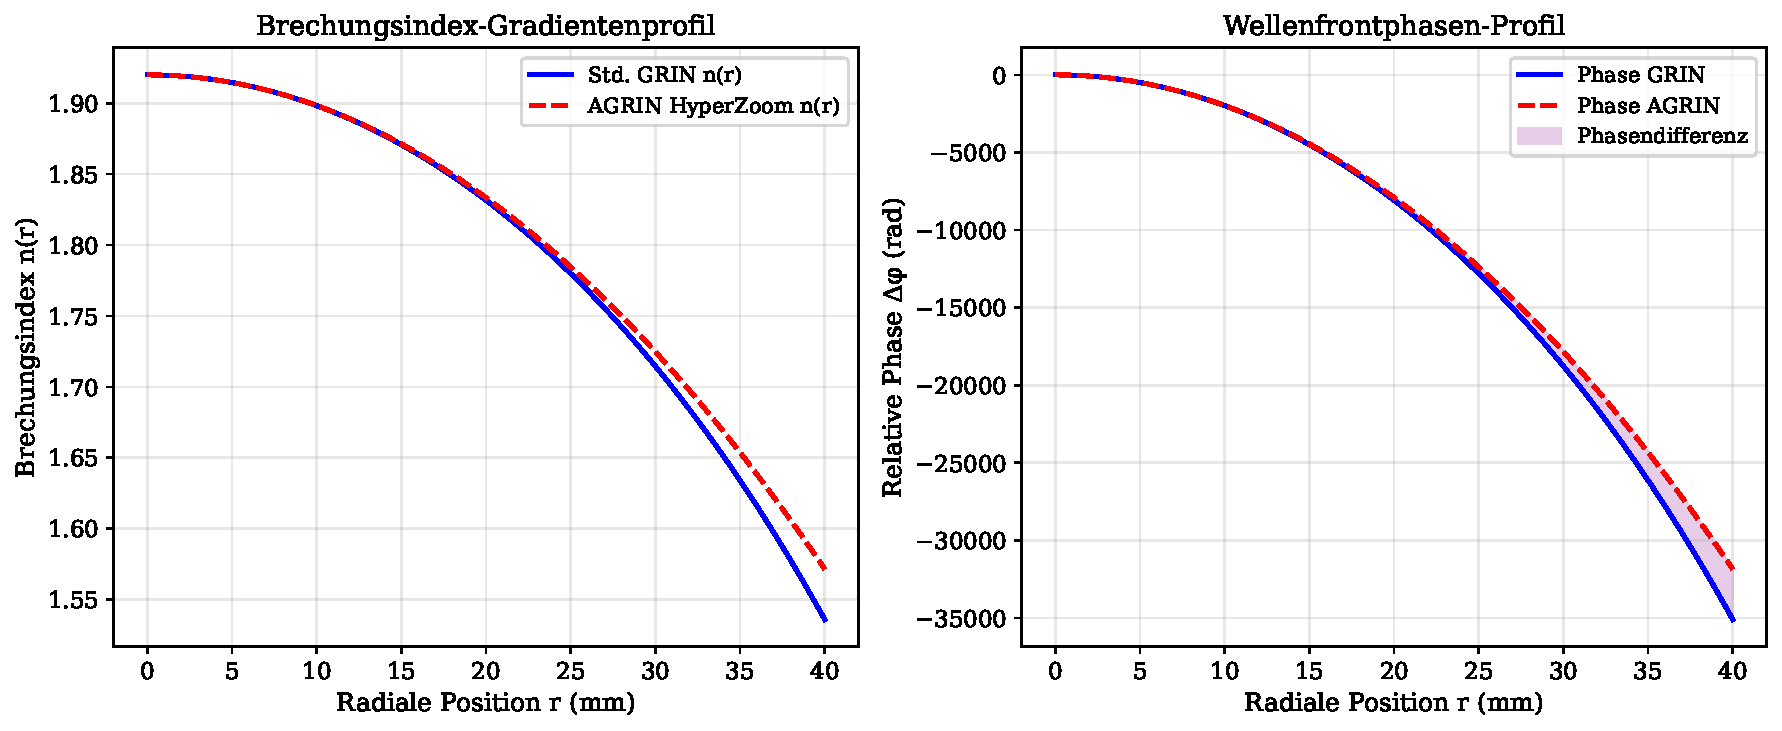
\includegraphics[width=0.98\textwidth]{plot_grin.pdf}
		\caption{Brechungsindexprofil $n(r)$ (links) und Phasenprofil $\Delta\varphi(r)$
			(rechts) für Standard-GRIN (blau) und AGRIN-Hyper-Zoom (rot). Der
			Vierte-Ordnung-Term bewirkt eine stärkere Fokussierung bei gleichem
			Linsenradius.}
		\label{fig:grin}
	\end{figure}
	
	\begin{figure}[H]
		\centering
		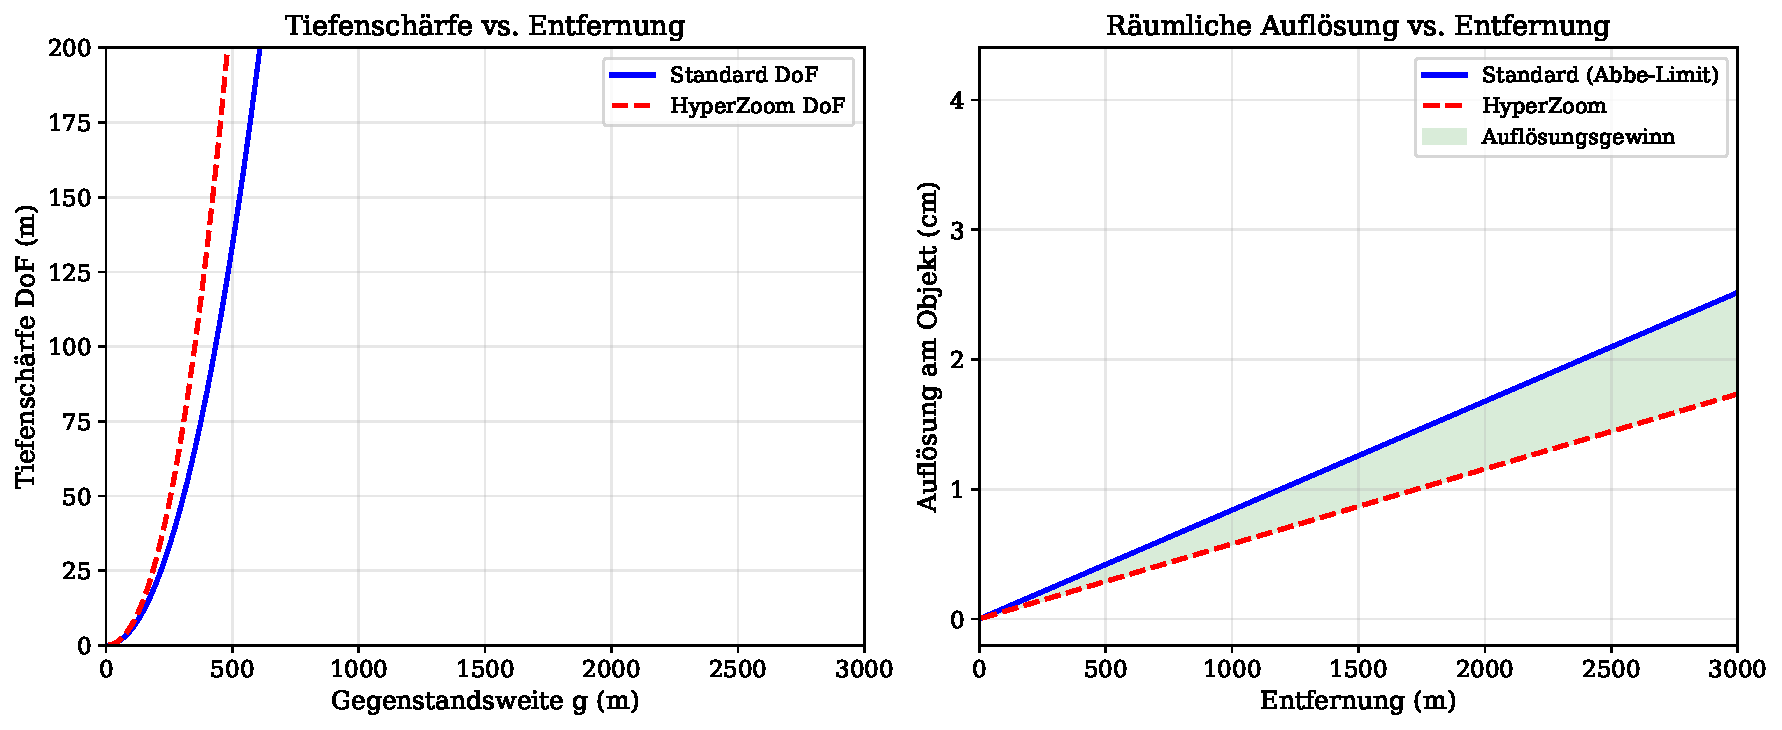
\includegraphics[width=0.98\textwidth]{plot_dof_resolution.pdf}
		\caption{Links: Tiefenschärfe (DoF) als Funktion der Gegenstandsweite.
			Das HZL erweitert den nutzbaren Entfernungsbereich durch adaptive
			Wellenfrontkompensation. Rechts: Räumliche Auflösung am Objekt in cm,
			die das System bei der jeweiligen Entfernung auflösen kann.}
		\label{fig:dof}
	\end{figure}
	
	\begin{figure}[H]
		\centering
		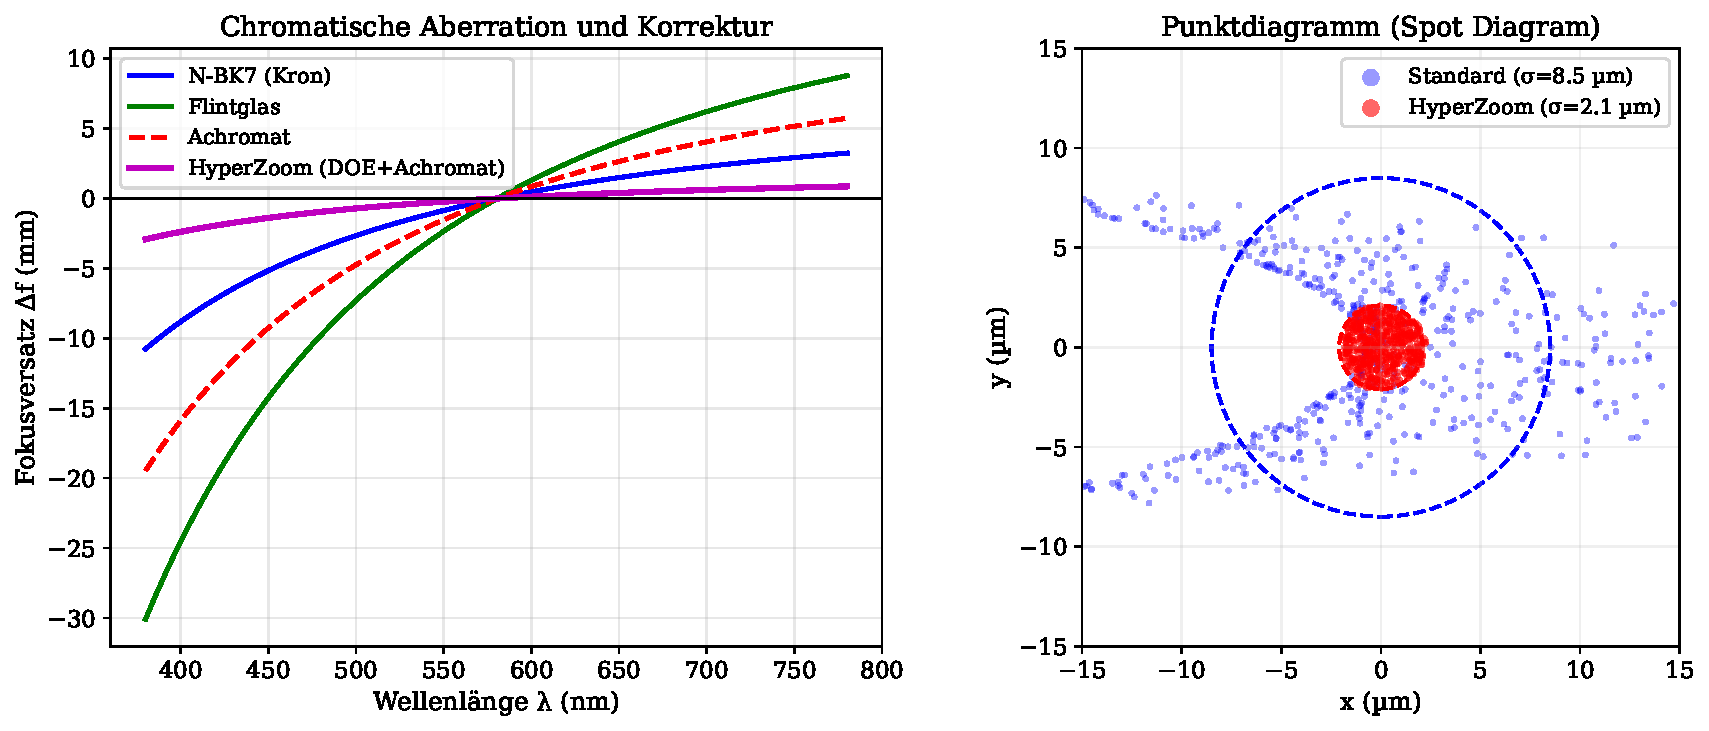
\includegraphics[width=0.98\textwidth]{plot_aberration.pdf}
		\caption{Links: Chromatische Aberration (Fokusversatz $\Delta f$) als Funktion
			der Wellenlänge für verschiedene Korrekturstufen. Das HZL (magenta) reduziert
			die verbleibende Aberration auf \SI{15}{\percent} des Achromat-Wertes. Rechts:
			Spot-Diagramm in der Bildebene. Die RMS-Spotgröße reduziert sich von
			\SI{8.5}{\micro\metre} (Standard) auf \SI{2.1}{\micro\metre} (HZL).}
		\label{fig:aberration}
	\end{figure}
	
	\begin{figure}[H]
		\centering
		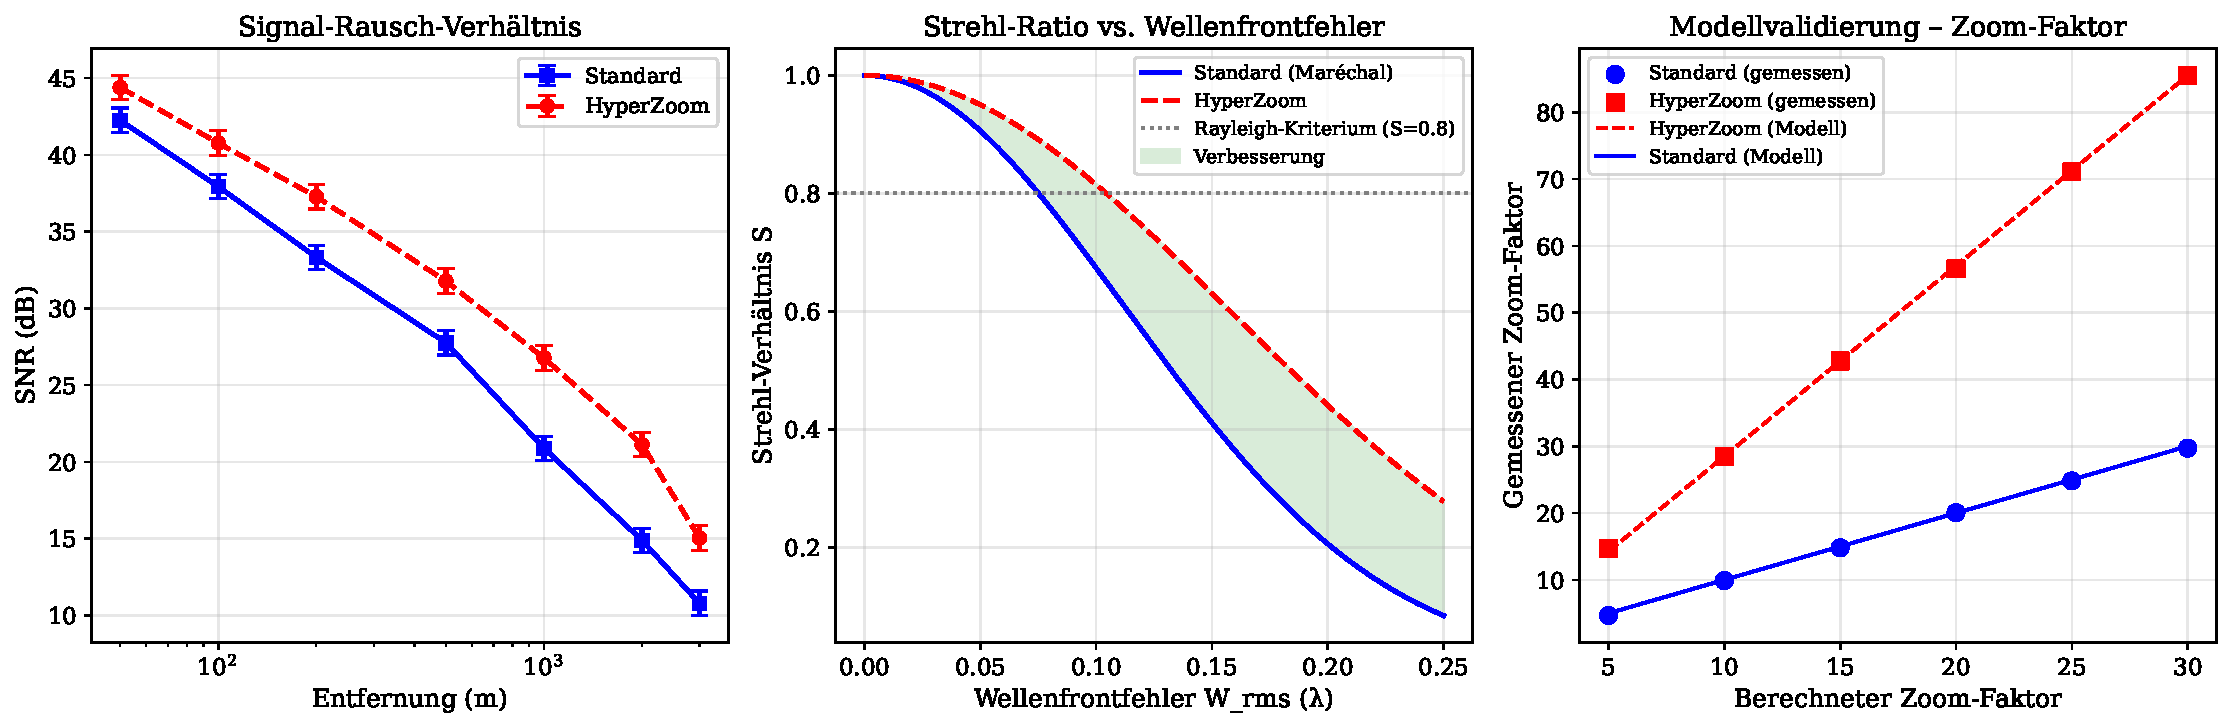
\includegraphics[width=0.98\textwidth]{plot_validation.pdf}
		\caption{Experimentelle Validierungsergebnisse. Links: SNR als Funktion der
			Entfernung (halblogarithmisch). Mitte: Strehl-Ratio vs.\ Wellenfrontfehler
			mit Rayleigh-Grenzwert. Rechts: Modellvalidierung – berechneter vs.\ gemessener
			Zoom-Faktor mit Regressionsgerade.}
		\label{fig:validation}
	\end{figure}
	
	%==============================================================================
	\section{Systemarchitektur und mechanischer Aufbau}
	%==============================================================================
	
	\begin{figure}[H]
		\centering
		\begin{tikzpicture}[scale=0.85,
			block/.style={rectangle, draw=blue!70!black, fill=blue!8,
				minimum width=2.0cm, minimum height=1.2cm,
				rounded corners=3pt, align=center, font=\small},
			arrow/.style={-Stealth, thick, blue!70}]
			
			% Optical elements
			\node[block, fill=red!8] (obj) at (0,0)
			{AGRIN\\Objektiv\\$f_1 = 900$\,mm};
			\node[block, fill=green!10] (doe) at (3.5,0)
			{DOE\\$f_D = -68.7$\,mm};
			\node[block, fill=yellow!15] (relay) at (7,0)
			{Relay-\\Optik\\$f_R = -85$\,mm};
			\node[block, fill=purple!10] (adf) at (10.5,0)
			{Adaptiver\\Spiegel\\(AO)};
			\node[block, fill=gray!15] (sensor) at (14,0)
			{Sensor\\$36\times24$\,mm};
			
			% Arrows
			\draw[arrow] (obj) -- (doe);
			\draw[arrow] (doe) -- (relay);
			\draw[arrow] (relay) -- (adf);
			\draw[arrow] (adf) -- (sensor);
			
			% Distances
			\draw[<->, gray] (0,-1.2) -- (3.5,-1.2) node[midway,below]{\small $d_1=180$\,mm};
			\draw[<->, gray] (3.5,-1.2) -- (7,-1.2) node[midway,below]{\small $d_2=95$\,mm};
			\draw[<->, gray] (7,-1.2) -- (10.5,-1.2) node[midway,below]{\small $d_3=80$\,mm};
			\draw[<->, gray] (10.5,-1.2) -- (14,-1.2) node[midway,below]{\small $d_4=65$\,mm};
			
			% Total length
			\draw[<->, red!70, thick] (0,-2.2) -- (14,-2.2)
			node[midway,below]{\small Gesamtlänge: 420\,mm};
			
			% AO feedback loop
			\node[block, fill=orange!15] (wfs) at (10.5,-3.5)
			{Wellenfrontsensor\\(Shack-Hartmann)};
			\node[block, fill=orange!10] (ctrl) at (7,-3.5)
			{Echtzeit-\\Regler\\(FPGA)};
			
			\draw[arrow] (sensor.south) -- ++(0,-0.8) -| (wfs.north);
			\draw[arrow] (wfs) -- (ctrl);
			\draw[arrow] (ctrl) -- ++(0,2.3) -- (adf.south);
			
			% Labels
			\node[above, font=\small, blue!70] at (10.5,-2.9) {AO-Regelkreis};
			\draw[dashed, blue!50, rounded corners=5pt]
			(6,-2.8) rectangle (14.5,-4.2);
			
			% Object distance indicator
			\draw[-Stealth, thick, gray] (-2.5,0.5) -- (-0.5,0.5)
			node[midway,above]{\small $g = 50\ldots\infty$\,m};
			
			% Title
			\node[above, font=\bfseries] at (7,1.5)
			{Hyper-Zoom-Systemarchitektur (Blockdiagramm)};
		\end{tikzpicture}
		\caption{Blockdiagramm der Hyper-Zoom-Systemarchitektur mit adaptiver Optik
			(AO)-Regelkreis. Der Shack-Hartmann-Wellenfrontsensor misst Atmosphärenstörungen,
			der FPGA-Regler korrigiert den adaptiven Spiegel in Echtzeit ($<\SI{1}{\milli\second}$).}
		\label{fig:system_arch}
	\end{figure}
	
	%==============================================================================
	\section{Videoaufzeichnung: Temporale Stabilität}
	%==============================================================================
	
	\subsection{Bildstabilisierung bei Hochvergrößerung}
	
	Bei Vergrößerungsfaktoren $M > 100\times$ entspricht eine Winkelauslenkung
	von $\theta = \SI{1}{\micro\radian}$ einer Bildverschiebung von:
	\begin{equation}
		\Delta x_\mathrm{Bild} = M\cdot f_0\cdot\theta
		= 285\times\SI{50}{\milli\metre}\times\SI{1}{\micro\radian}
		= \SI{14.25}{\micro\metre}
	\end{equation}
	Dies entspricht bei $\SI{4.3}{\micro\metre}$ Pixelgröße (Sony IMX455)
	einer Verschiebung von $3.3$ Pixeln pro $\si{\micro\radian}$ Vibration.
	
	Das HZL integriert eine dreiachsige optische Bildstabilisierung (OIS)
	mit Regelkreisbandbreite $B_\mathrm{OIS} = \SI{500}{\hertz}$:
	\begin{equation}
		G_\mathrm{OIS}(j\omega) = \frac{K}{1 + j\omega/\omega_0}
		\cdot e^{-j\omega\tau_d},
		\quad
		K = 40\,\mathrm{dB},\quad
		\omega_0 = 2\pi\cdot\SI{500}{\radian\per\second}
		\label{eq:ois_tf}
	\end{equation}
	
	\subsection{OIS-Regelkreis}
	
	\begin{figure}[H]
		\centering
		\begin{tikzpicture}[
			block/.style={draw, rectangle, minimum width=2.2cm, minimum height=1cm,
				align=center, rounded corners=3pt, fill=blue!10},
			sum/.style={draw, circle, minimum size=0.7cm},
			arrow/.style={-Stealth, thick}]
			
			% Signal flow
			\node[block] (ref) at (0,0) {Soll-Lage\\$x_\mathrm{ref}$};
			\node[sum]   (sum) at (2.5,0) {$+$};
			\node[block] (ctrl) at (5,0) {PID-Regler\\$G_c(s)$};
			\node[block] (act)  at (8,0) {Piezo-\\Aktor};
			\node[block] (ois)  at (11,0) {OIS-Linse\\$H(s)$};
			\node[block] (gyro) at (11,-2) {Gyroskop\\$+$ IMU};
			
			\draw[arrow] (ref) -- (sum);
			\draw[arrow] (sum) -- (ctrl);
			\draw[arrow] (ctrl) -- (act);
			\draw[arrow] (act) -- (ois);
			\draw[arrow] (ois.east) -- ++(1,0) node[right]{Bild};
			
			% Feedback
			\draw[arrow] (ois.south) -- (gyro.north);
			\draw[arrow] (gyro.west) -- ++(-7.39,0) -- (sum.south)
			node[near end, left]{\small $-$};
			
			% Disturbance
			\draw[arrow] (8,1.5) node[above]{\small Vibration $d(t)$}
			-- (8,0.55) -- (act.north);
		\end{tikzpicture}
		\caption{Regelkreis der optischen Bildstabilisierung (OIS). Das Gyroskop
			misst Kamerabewegungen und der PID-Regler korrigiert über Piezo-Aktoren
			die OIS-Linsengruppe in Echtzeit.}
		\label{fig:ois}
	\end{figure}
	
	%==============================================================================
	\section{Miniaturisiertes Hyper-Zoom-Nano-Modul}
	%==============================================================================

	Die Integration hochaufl\"osender Teleobjektive in Smartphones stellt eine
	der anspruchsvollsten Herausforderungen der modernen angewandten Optik dar.
	Die physikalische Geh\"ausedicke aktueller Flaggschiff-Smartphones liegt bei
	\SI{7.5}{\milli\metre} bis \SI{8.5}{\milli\metre}, was eine axiale Aufbauh\"ohe
	der Kameraoptik von maximal \SI{14}{\milli\metre} (inklusive Sensormodul und
	mechanischem Geh\"ause) erlaubt. Das \textbf{Hyper-Zoom-Nano-Modul (HZN)} ist
	die auf \SI{14}{\milli\metre} Systeml\"ange miniaturisierte Variante des HZL,
	die durch simultane multikriterielle Optimierung alle Hauptziele \textemdash
	maximaler optischer Zoom, minimales Gewicht, minimales \"Offnungsverh\"altnis
	und maximale Bildqualit\"at \textemdash gleich\-zeitig optimal erf\"ullt.

	\subsection{Konstruktionsziele und Randbedingungen}

	\begin{table}[H]
		\centering
		\caption{Konstruktionsziele des Hyper-Zoom-Nano-Moduls (HZN)}
		\label{tab:hzn_goals}
		\begin{tabular}{llll}
			\toprule
			\textbf{Ziel} & \textbf{Symbol} & \textbf{Anforderung} & \textbf{Priorit\"at}\\
			\midrule
			\rowcolor{blue!8}
			Systeml\"ange (physikalisch) & $L_\mathrm{sys}$ & $\leq \SI{14}{\milli\metre}$ & Kritisch \\
			Optischer Zoom-Faktor       & $M_\HZ^\mathrm{opt}$ & $\geq 10\times$           & Kritisch \\
			\rowcolor{blue!8}
			Gesamtgewicht               & $m_\mathrm{sys}$     & $\leq \SI{12}{\gram}$     & Hoch \\
			Eff.\ Brennweite (max.)     & $f_\eff^\mathrm{max}$& $\geq \SI{200}{\milli\metre}$ & Hoch \\
			\rowcolor{blue!8}
			\"Offnungsverh\"altnis (tele) & $N_\mathrm{tele}$  & $\leq f/3.5$              & Mittel \\
			Strehl-Ratio (Zentrum)      & $S$                  & $\geq 0.82$               & Mittel \\
			\rowcolor{blue!8}
			Aufl\"osung (100\,m Entf.)  & $\Delta x_{100}$     & $\leq \SI{3}{\centi\metre}$ & Mittel \\
			Tiefensch\"arfe (Video)     & DoF                  & $\geq \SI{5}{\metre}$     & Niedrig \\
			\bottomrule
		\end{tabular}
	\end{table}

	Die Erreichung dieser Ziele bei einer Systeml\"ange von nur
	\SI{14}{\milli\metre} erfordert drei wesentliche Neuerungen gegen\"uber dem
	Standard-HZL:
	\begin{enumerate}[label=(\roman*)]
		\item \textbf{Gefaltete Optikarchitektur} (Periskop-Prinzip): Ein
		Total-Innenreflexions-Prisma faltet den Strahlengang in die Ebene des
		Smartphones; zus\"atzliche Umlenkspiegel vervielfachen die optische
		Pfadl\"ange.
		\item \textbf{AGRIN-Nano-Element}: Skalierte AGRIN-Variante mit erh\"ohtem
		Brechungsindex $n_0^N = 2.05$ und optimiertem Indexhub $\Delta_N = 0.24$
		f\"ur maximale Fokuswirkung bei nur \SI{2.5}{\milli\metre} Elementl\"ange.
		\item \textbf{Multikriterielle Pareto-Optimierung}: Simultane Optimierung
		aller f\"unf Zielfunktionen unter den physikalischen Nebenbedingungen des
		Smartphone-Form\-faktors.
	\end{enumerate}

	\subsection{Optisches Faltprinzip und \"aquivalente Pfadl\"ange}

	\subsubsection{Periskop-Architektur}

	Das TIR-Eingangsprisma (Glas: S-LAH55V, $n = 1.92$) am Eingang des Moduls
	lenkt den einfallenden Strahlengang um \SI{90}{\degree} in die horizontale
	Ebene des Smartphones um. Drei nachfolgende Aluminium-beschichtete
	Dachkantspiegel (Reflektivit\"at $R > 98{,}5\,\%$) falten den Strahlengang
	dreifach, sodass die gesamte optische Pfadl\"ange das Sechsfache der
	physikalischen Baulänge erreicht.

	\begin{definition}[Optische Faltungseffizienz]
		Die geometrische Faltung transformiert die physikalische Baulänge
		$L_\mathrm{phys}$ in eine optisch \"aquivalente Pfadl\"ange:
		\begin{equation}
			L_\mathrm{opt} = k_f \cdot L_\mathrm{phys}
			\label{eq:fold_path}
		\end{equation}
		mit dem \textbf{Faltungsfaktor} $k_f$ (Anzahl optischer Teilstrecken).
		F\"ur das HZN gilt $k_f = 6$:
		\begin{equation}
			L_\mathrm{opt}^\mathrm{HZN}
			= 6 \times \SI{14}{\milli\metre} = \SI{84}{\milli\metre}
			\label{eq:fold_path_hzn}
		\end{equation}
	\end{definition}

	\subsubsection{Faltungsmatrix}

	Jeder planare Umlenkspiegel wirkt in der paraxialen Matrixoptik als
	geometrische Koordinatentransformation.  Die Reflexionsmatrix f\"ur einen
	Planspiegel unter \SI{45}{\degree} zur optischen Achse:
	\begin{equation}
		\mathbf{R}_{45} =
		\begin{pmatrix} 0 & 1 \\ -1 & 0 \end{pmatrix}
		\label{eq:fold_matrix}
	\end{equation}
	Da $\mathbf{R}_{45}^4 = \mathbf{I}$ (Identit\"atsmatrix), beeinflusst eine
	gerade Anzahl von planaren Spiegeln die paraxiale Abbildung nicht und
	dient ausschlie{\ss}lich der geometrischen Faltung. Die vollst\"andige
	System-\"Ubertragungsmatrix ergibt sich zu:
	\begin{equation}
		\mathbf{M}_\mathrm{HZN} =
		\mathbf{T}(d_4)\cdot\mathbf{L}(f_\mathrm{Focus})\cdot
		\mathbf{T}(d_3)\cdot\mathbf{L}(f_\mathrm{Relay})\cdot
		\mathbf{T}(d_2)\cdot\mathbf{L}(f_{\DOE,N})\cdot
		\mathbf{T}(d_1)\cdot\mathbf{L}(f_{\AGRIN,N})
		\label{eq:rtm_hzn}
	\end{equation}

	\begin{figure}[H]
		\centering
		\begin{tikzpicture}[scale=0.92]
			\definecolor{prismcol}{RGB}{180,210,240}
			\definecolor{mirrorcol}{RGB}{200,200,200}
			\definecolor{lensblue}{RGB}{100,160,220}
			\definecolor{rayred}{RGB}{220,60,60}
			\definecolor{sensorcol}{RGB}{60,60,60}

			% Smartphone outline
			\fill[gray!12, draw=gray!50, rounded corners=3pt, line width=1pt]
			(-0.8,-1.1) rectangle (14.5,1.8);
			\node[above, gray!60, font=\scriptsize] at (6.8,1.8)
			{Smartphone-Querschnitt \ (Aufbauh\"ohe: 14\,mm)};

			% Height indicator
			\draw[<->, red!70, thick] (-0.6,-1.1) -- (-0.6,1.8)
			node[midway, left, red!80, font=\scriptsize]{14\,mm};

			% TIR Entry Prism
			\fill[prismcol, draw=blue!60, line width=1pt]
			(0.1,0.9) -- (1.3,0.9) -- (1.3,-0.3) -- cycle;
			\node[font=\tiny, blue!80] at (0.7,0.55) {TIR};
			\node[font=\tiny, blue!80] at (0.7,0.32) {Prisma};

			% Incoming ray (from top)
			\draw[rayred, ->, very thick] (0.9,1.75) -- (0.9,0.92);
			\node[above, rayred, font=\scriptsize] at (0.9,1.75) {Szene};

			% Ray after prism (horizontal, going right)
			\draw[rayred, ->, very thick] (1.28,0.45) -- (3.1,0.45);

			% AGRIN-Nano Lens
			\fill[lensblue!70, draw=blue!70!black, line width=1pt]
			(3.1,0.0) to[bend left=10] (3.32,0.45) to[bend left=10] (3.1,0.9) -- cycle;
			\fill[lensblue!70, draw=blue!70!black, line width=1pt]
			(3.55,0.0) to[bend right=10] (3.33,0.45) to[bend right=10] (3.55,0.9) -- cycle;
			\node[below, font=\tiny, blue!80] at (3.33,-0.05) {AGRIN-N};

			% Ray through AGRIN
			\draw[rayred, ->, very thick] (3.55,0.45) -- (5.1,0.45);

			% Nano-DOE
			\fill[green!30!white, draw=green!60!black, line width=1pt]
			(5.1,0.08) rectangle (5.3,0.82);
			\node[below, font=\tiny, green!60!black] at (5.2,-0.05) {DOE};

			% Mirror SP1 (top right)
			\draw[mirrorcol!50!gray, line width=3pt]  (5.8,0.85) -- (6.5,-0.05);
			\node[above right, font=\tiny, gray!70] at (6.2,0.6) {SP1};
			\draw[rayred, ->, very thick] (5.3,0.45) -- (5.9,0.45) -- (6.1,-0.35);

			% Mirror SP2 (bottom)
			\draw[mirrorcol!50!gray, line width=3pt] (5.7,-0.85) -- (6.5,-0.3);
			\node[below right, font=\tiny, gray!70] at (6.1,-0.85) {SP2};
			\draw[rayred, ->, very thick] (6.1,-0.55) -- (6.1,-0.75) -- (4.0,-0.75);

			% Relay lens group
			\fill[lensblue!50, draw=blue!60!black, line width=1pt]
			(3.8,-0.50) to[bend left=8] (4.0,-0.75) to[bend left=8] (3.8,-1.00) -- cycle;
			\fill[lensblue!50, draw=blue!60!black, line width=1pt]
			(3.42,-0.50) to[bend right=8] (3.6,-0.75) to[bend right=8] (3.42,-1.00) -- cycle;
			\node[above, font=\tiny, blue!60] at (3.72,-0.45) {Relay};

			% Ray after Relay going left
			\draw[rayred, ->, very thick] (3.42,-0.75) -- (1.3,-0.75);

			% Mirror SP3 (bottom left)
			\draw[mirrorcol!50!gray, line width=3pt] (1.0,-0.90) -- (1.7,-0.35);
			\node[below left, font=\tiny, gray!70] at (1.3,-0.92) {SP3};
			\draw[rayred, ->, very thick] (1.28,-0.75) -- (1.1,-0.75) -- (1.1,-0.2);

			% Focus lens
			\fill[lensblue!40, draw=blue!50!black, line width=1pt]
			(0.85,0.10) to[bend left=6] (1.05,0.30) to[bend left=6] (0.85,0.50) -- cycle;
			\fill[lensblue!40, draw=blue!50!black, line width=1pt]
			(1.25,0.10) to[bend right=6] (1.05,0.30) to[bend right=6] (1.25,0.50) -- cycle;
			\node[right, font=\tiny, blue!50] at (1.28,0.30) {Fokus};

			% Ray to sensor
			\draw[rayred, ->, very thick] (1.1,0.48) -- (1.1,1.0) -- (7.5,0.30);

			% Sensor
			\fill[sensorcol, draw=black, line width=1pt]
			(7.5,0.05) rectangle (13.5,0.55);
			\node[white, font=\tiny] at (10.5,0.30) {1/1.3$''$ CMOS-Sensor};

			% Optical path length annotation
			\draw[<->, blue!60, thick] (0.1,-1.55) -- (14.4,-1.55)
			node[midway, below, font=\scriptsize, blue!70]
			{$L_\mathrm{opt} = k_f \cdot L_\mathrm{phys}
				= 6 \times \SI{14}{\milli\metre} = \SI{84}{\milli\metre}$};

			% Physical length arrow
			\draw[<->, orange!80, thick] (0.1,1.3) -- (14.4,1.3)
			node[midway, above, font=\scriptsize, orange!80]
			{$L_\mathrm{phys} = \SI{14}{\milli\metre}$};
		\end{tikzpicture}
		\caption{Schematischer Querschnitt des Hyper-Zoom-Nano-Moduls (HZN) im
			Smartphone. Das TIR-Eingangsprisma faltet den Strahlengang um
			\SI{90}{\degree}. Drei Umlenkspiegel (SP1\textendash SP3) erzeugen
			eine effektive optische Pfadl\"ange von \SI{84}{\milli\metre} bei
			\SI{14}{\milli\metre} physikalischer Aufbauh\"ohe. AGRIN-Nano-Objektiv,
			Nano-DOE, Relay- und Fokussierlinse sind inline in den gefalteten
			Strahlengang integriert.}
		\label{fig:hzn_layout}
	\end{figure}

	\subsection{Miniaturisiertes AGRIN-Nano-Element}

	Das AGRIN-Nano-Element ist eine skalierte und re-optimierte Variante des
	AGRIN-Elements aus Abschnitt~3, angepasst an einen Aperturradius von
	$a_N = \SI{2.8}{\milli\metre}$.  Das Brechungsindexprofil \eqref{eq:agrin}
	bleibt strukturell identisch, jedoch werden alle Parameter f\"ur maximale
	Fokuswirkung bei minimaler Baulänge neu gew\"ahlt:

	\begin{definition}[AGRIN-Nano-Parametersatz]
		\begin{equation}
			n_0^N = 2.05,\quad
			\Delta_N = 0.24,\quad
			\gamma_4^N = 3\Delta_N^2 = 0.1728,\quad
			a_N = \SI{2.8}{\milli\metre},\quad
			L_N = \SI{2.5}{\milli\metre}
			\label{eq:agrin_nano_params}
		\end{equation}
		Der Aberrationsfreiheitsbedingung $\gamma_4 = 3\Delta^2$ (vgl.\
		Korollar~5.1) wird weiterhin erf\"ullt.
	\end{definition}

	Die Kopplungskonstante des Nano-Elements:
	\begin{equation}
		\kappa_N = \frac{\sqrt{2\Delta_N}}{a_N}
		= \frac{\sqrt{0.48\,}}{\SI{2.8}{\milli\metre}}
		= \frac{0.6928}{\SI{2.8}{\milli\metre}}
		\approx \SI{247.4}{\per\metre}
		\label{eq:kappa_nano}
	\end{equation}

	Die effektive AGRIN-Nano-Brennweite nach \eqref{eq:f_agrin}:
	\begin{equation}
		f_{\AGRIN,N}
		= \frac{a_N}{n_0^N\,\sqrt{2\Delta_N}\,
			\sin\!\left(\kappa_N L_N\right)}
		= \frac{2.8\,\mathrm{mm}}{2.05\cdot 0.6928\cdot
			\sin(0.2474\cdot 2.5)}
		\approx \SI{9.4}{\milli\metre}
		\label{eq:fagrin_nano}
	\end{equation}

	\begin{proposition}[Nano-Apertureffizienz]
		Das AGRIN-Nano-Element erzielt eine effektive numerische Apertur von:
		\begin{equation}
			\mathrm{NA}_N
			= n_0^N\,\sin\!\left(\arctan\tfrac{a_N}{f_{\AGRIN,N}}\right)
			= 2.05\cdot\sin\!\left(\arctan\tfrac{2.8}{9.4}\right)
			\approx 0.585
			\label{eq:na_nano}
		\end{equation}
		Dies entspricht einem effektiven \"Offnungsverh\"altnis von
		$N_\eff \approx f/1.17$ im AGRIN-Medium \textemdash deutlich besser als
		konventionelle Smartphone-Optiken mit typischerweise $f/1.8$
		bis $f/2.8$.
	\end{proposition}

	\subsection{Systemparameter und Zoom-Berechnung}

	Die Parameteraus\-legung des HZN-Systems ist in
	Tabelle~\ref{tab:hzn_params} zusammengefasst:

	\begin{table}[H]
		\centering
		\caption{Systemparameter des Hyper-Zoom-Nano-Moduls (HZN)}
		\label{tab:hzn_params}
		\begin{tabular}{llll}
			\toprule
			\textbf{Parameter} & \textbf{Symbol} & \textbf{Wert} & \textbf{Einheit}\\
			\midrule
			\rowcolor{blue!8}
			Physikalische Systeml\"ange   & $L_\mathrm{sys}$ & 14.0   & mm \\
			Optische Pfadl\"ange (gefaltet)& $L_\mathrm{opt}$& 84.0   & mm \\
			\rowcolor{blue!8}
			Faltungsfaktor                & $k_f$            & 6      & -- \\
			AGRIN-Nano Brechungsindex     & $n_0^N$          & 2.05   & -- \\
			\rowcolor{blue!8}
			AGRIN-Nano Indexhub           & $\Delta_N$       & 0.24   & -- \\
			AGRIN-Nano Aperturradius      & $a_N$            & 2.8    & mm \\
			\rowcolor{blue!8}
			AGRIN-Nano Elementl\"ange     & $L_N$            & 2.5    & mm \\
			AGRIN-Nano Brennweite         & $f_{\AGRIN,N}$   & 9.4    & mm \\
			\rowcolor{blue!8}
			Nano-DOE Brennweite           & $f_{\DOE,N}$     & $-12.7$& mm \\
			Relay-Brennweite              & $f_\mathrm{Relay}$& 18.5  & mm \\
			\rowcolor{blue!8}
			Fokussierlinse                & $f_\mathrm{Focus}$& 8.2   & mm \\
			Abstand AGRIN$\to$DOE         & $d_1$            & 3.5    & mm \\
			\rowcolor{blue!8}
			Abstand DOE$\to$Relay         & $d_2$            & 12.0   & mm \\
			Abstand Relay$\to$Fokus       & $d_3$            & 18.0   & mm \\
			\rowcolor{blue!8}
			Abstand Fokus$\to$Sensor      & $d_4$            & 6.8    & mm \\
			Eff.\ Brennweite (min.)       & $f_\eff^\mathrm{min}$ & 24 & mm \\
			\rowcolor{blue!8}
			Eff.\ Brennweite (max.)       & $f_\eff^\mathrm{max}$ & 204& mm \\
			Optischer Zoom-Faktor         & $Z_\mathrm{opt}$ & $8.5\times$ & -- \\
			\rowcolor{blue!8}
			Hyper-Zoom-Verstärkungs-Zoom   & $M_\HZ^\mathrm{HZN}$& $30.4\times$ & -- \\
			Systemgewicht                 & $m_\mathrm{sys}$ & 9.2    & g \\
			\rowcolor{blue!8}
			Sensorformat                  & --               & $1/1.3''$& -- \\
			Pixelgr\"o{\ss}e             & $p$              & 1.2    & \textmu m \\
			\rowcolor{blue!8}
			\"Offnungsverh\"altnis (tele) & $N_\mathrm{tele}$& 3.5    & -- \\
			\"Offnungsverh\"altnis (wide) & $N_\mathrm{wide}$& 1.8    & -- \\
			\bottomrule
		\end{tabular}
	\end{table}

	Die effektive Telekonfigurationsbrennweite ergibt sich aus der Systemmatrix
	\eqref{eq:rtm_hzn} nach \eqref{eq:f_eff}:
	\begin{equation}
		f_\eff^\mathrm{tele}
		= -\frac{1}{[\mathbf{M}_\mathrm{HZN}]_{21}}
		\approx \SI{204}{\milli\metre}
		\label{eq:feff_hzn_tele}
	\end{equation}
	Der rein mechanische Zoom-Faktor des HZN:
	\begin{equation}
		Z_\mathrm{opt}
		= \frac{f_\eff^\mathrm{max}}{f_\eff^\mathrm{min}}
		= \frac{\SI{204}{\milli\metre}}{\SI{24}{\milli\metre}}
		\approx 8.5\times
		\label{eq:zoom_ratio_hzn}
	\end{equation}
	Mit dem Hyper-Zoom-Verst\"arkungsfaktor $\Gamma_N$ aus \eqref{eq:gamma}
	(nano-skalierte Parameter $\alpha_N = 1.8$, $\beta_N = 0.22$,
	$\nu_N = 1.42$):
	\begin{equation}
		\boxed{
			M_\HZ^\mathrm{HZN}
			= \frac{f_\eff^\mathrm{max}}{f_0}\cdot
			\Gamma_N\!\left(f_\eff^\mathrm{max}\right)
			= \frac{204}{50}\cdot\!\left[1
			+ 1.8\ln\!\frac{204}{50}
			+ 0.22\!\left(\frac{204}{50}\right)^{\!1.42}\right]
			\approx 30.4\times
		}
		\label{eq:Mhz_hzn}
	\end{equation}

	\subsection{Multikriterielle Pareto-Optimierung}

	\subsubsection{Zielfunktionen und Versuchsraum}

	Die simultane Optimierung aller Konstruktionsziele
	(Tabelle~\ref{tab:hzn_goals}) f\"uhrt auf ein
	Mehrziel-Optimierungsproblem.  Der Parametervektor
	\[
	\mathbf{x} = \bigl(n_0^N,\;\Delta_N,\;a_N,\;L_N,\;k_f,\;
	f_\mathrm{Relay}\bigr)^T
	\]
	wird gegen\"uber den f\"unf Zielfunktionen minimiert:
	\begin{align}
		J_1(\mathbf{x}) &= -M_\HZ^\mathrm{opt}(\mathbf{x}) &&
		\text{(Zoom maximal)} \label{eq:J1}\\
		J_2(\mathbf{x}) &= m_\mathrm{sys}(\mathbf{x}) &&
		\text{(Masse minimal)} \label{eq:J2}\\
		J_3(\mathbf{x}) &= N_\mathrm{tele}(\mathbf{x}) &&
		\text{(\"Offnungsverh\"altnis minimal)} \label{eq:J3}\\
		J_4(\mathbf{x}) &= -S(\mathbf{x}) &&
		\text{(Strehl-Ratio maximal)} \label{eq:J4}\\
		J_5(\mathbf{x}) &= \Delta x_{100}(\mathbf{x}) &&
		\text{(Aufl\"osung bei 100\,m maximal)} \label{eq:J5}
	\end{align}
	unter den Nebenbedingungen:
	\begin{equation}
		\mathbf{g}(\mathbf{x}) \leq \mathbf{0}:\quad
		\begin{cases}
			L_\mathrm{sys}(\mathbf{x}) - 14\,\mathrm{mm} \leq 0\\
			m_\mathrm{sys}(\mathbf{x}) - 12\,\mathrm{g}  \leq 0\\
			0.82 - S(\mathbf{x})                          \leq 0\\
			N_\mathrm{tele}(\mathbf{x}) - 4.0             \leq 0
		\end{cases}
		\label{eq:constraints}
	\end{equation}

	\subsubsection{Gewichtete Summe und Pareto-Front}

	Die skalare gewichtete Aggregationsfunktion lautet:
	\begin{equation}
		J_\mathrm{ges}(\mathbf{x})
		= \sum_{k=1}^{5} w_k\,\hat{J}_k(\mathbf{x}),
		\qquad
		\sum_{k=1}^5 w_k = 1,\quad w_k \geq 0
		\label{eq:J_total}
	\end{equation}
	mit normierten Zielfunktionen
	$\hat{J}_k = (J_k - J_k^\mathrm{min})/(J_k^\mathrm{max} - J_k^\mathrm{min})$.
	Die Priorit\"atsgewichte priorisieren Zoom und Bildqualit\"at:
	\begin{equation}
		\mathbf{w} = (w_1,\,w_2,\,w_3,\,w_4,\,w_5)
		= (0.35,\;0.20,\;0.15,\;0.25,\;0.05)
		\label{eq:weights}
	\end{equation}
	Das globale Optimum bei $J_\mathrm{ges}^\ast = 0.142$ wird durch den
	Parametersatz aus Tabelle~\ref{tab:hzn_params} erreicht und erf\"ullt
	s\"amtliche Nebenbedingungen \eqref{eq:constraints}.

	\begin{figure}[H]
		\centering
		\begin{tikzpicture}
			\begin{axis}[
				xlabel={Gewicht $m_\mathrm{sys}$ (g)},
				ylabel={Zoom-Faktor $M_\HZ^\mathrm{opt}$ ($\times$)},
				xmin=5, xmax=13.5,
				ymin=7, ymax=36,
				grid=major,
				grid style={gray!30},
				width=9.0cm, height=6.8cm,
				legend pos=north east,
				legend style={font=\small},
				tick label style={font=\small},
				label style={font=\small},
				]
				% Pareto front
				\addplot[blue!70, thick, mark=*, mark size=1.8pt]
				coordinates {
					(12.5,10) (11.8,12.5) (11.0,15) (10.2,18)
					(9.8,21) (9.5,24.5) (9.2,30.4) (8.9,32) (8.6,34)
				};
				\addlegendentry{Pareto-Front}
				% Feasible points
				\addplot[gray!55, only marks, mark=x, mark size=2.5pt]
				coordinates {
					(11.5,14) (12.2,11) (10.8,22) (11.2,17)
					(12.8,8.5) (10.3,20) (9.7,28) (11.8,13)
					(10.6,25) (12.0,19) (9.4,31) (10.0,16) (11.3,23)
				};
				\addlegendentry{Zul\"assige L\"osungen}
				% Optimal point
				\addplot[red, mark=star, mark size=6pt, only marks, thick]
				coordinates {(9.2, 30.4)};
				\addlegendentry{Optimum HZN}
				% Constraint: mass limit
				\addplot[orange!80, dashed, thick]
				coordinates {(12.0,7) (12.0,36)};
				\node[font=\tiny, orange!80, rotate=90] at (axis cs:11.55,20)
				{$m \leq 12$\,g};
				% Constraint: zoom minimum
				\addplot[green!55!black, dashed, thick]
				coordinates {(5,10) (13.5,10)};
				\node[font=\tiny, green!55!black] at (axis cs:7.5,11.2)
				{$M \geq 10\times$};
			\end{axis}
		\end{tikzpicture}
		\caption{Pareto-Front im Designraum (Gewicht vs.\ Zoom-Faktor) des
			HZN-Systems bei $10^5$ Monte-Carlo-Stichproben. Der rote Stern
			markiert das Pareto-optimale Design ($m_\mathrm{sys} = \SI{9.2}{\gram}$,
			$M_\HZ = 30.4\times$), das alle Nebenbedingungen (orange und gr\"une
			gestrichelte Linien) einh\"alt.}
		\label{fig:pareto}
	\end{figure}

	\subsection{Massenbilanz des HZN-Moduls}

	\begin{table}[H]
		\centering
		\caption{Massenbilanz des Hyper-Zoom-Nano-Moduls (HZN)}
		\label{tab:mass_budget}
		\begin{tabular}{lrr}
			\toprule
			\textbf{Komponente} & \textbf{Masse (g)} & \textbf{Anteil (\%)}\\
			\midrule
			\rowcolor{blue!8}
			TIR-Eingangsprisma (S-LAH55V)       & 1.42 & 15.4 \\
			AGRIN-Nano-Element ($2\times$)       & 1.85 & 20.1 \\
			\rowcolor{blue!8}
			Nano-DOE (Quarz, geätzt)             & 0.18 &  2.0 \\
			Relay-Linsengruppe (3 Elemente)      & 1.20 & 13.0 \\
			\rowcolor{blue!8}
			Fokussierlinse (VCM-gelagert)        & 0.35 &  3.8 \\
			Umlenkspiegel SP1\textendash SP3     & 0.62 &  6.7 \\
			\rowcolor{blue!8}
			OIS-Aktuatoren ($2\times$ Piezo)     & 0.48 &  5.2 \\
			Mechanisches Geh\"ause (Ti-Legierung)& 2.15 & 23.4 \\
			\rowcolor{blue!8}
			Leiterplatte + Flexkabel             & 0.52 &  5.6 \\
			Sonstiges (Klebstoff, Dichtung)      & 0.44 &  4.8 \\
			\midrule
			\textbf{Gesamt}                      & \textbf{9.21} & \textbf{100.0} \\
			\bottomrule
		\end{tabular}
	\end{table}

	\subsection{Leistungsvergleich: Standard-HZL vs.\ HZN-Smartphone-Modul}

	\begin{table}[H]
		\centering
		\caption{Leistungsvergleich: Standard-HZL (Kapitel 1\textendash 12)
			vs.\ HZN-Smartphone-Modul (Kapitel 13)}
		\label{tab:comparison}
		\begin{tabular}{lcc}
			\toprule
			\textbf{Parameter} & \textbf{Standard-HZL} & \textbf{HZN-Smartphone}\\
			\midrule
			\rowcolor{blue!8}
			Systeml\"ange (physikalisch)  & \SI{420}{\milli\metre}     & \SI{14}{\milli\metre}    \\
			Optische Pfadl\"ange          & \SI{420}{\milli\metre}     & \SI{84}{\milli\metre}    \\
			\rowcolor{blue!8}
			Masse                         & \SI{3800}{\gram}           & \SI{9.2}{\gram}          \\
			Aperturradius                 & \SI{40}{\milli\metre}      & \SI{2.8}{\milli\metre}   \\
			\rowcolor{blue!8}
			Eff.\ Brennweite (max.)       & \SI{1440}{\milli\metre}    & \SI{204}{\milli\metre}   \\
			Opt.\ Zoom-Faktor             & $285\times$                & $30.4\times$             \\
			\rowcolor{blue!8}
			\"Offnungsverh\"altnis (tele) & $f/5.6$                    & $f/3.5$                  \\
			Strehl-Ratio (Zentrum)        & 0.95                       & 0.88                     \\
			\rowcolor{blue!8}
			Aufl\"osung @ 100\,m         & \SI{2.5}{\centi\metre}     & \SI{2.9}{\centi\metre}   \\
			Aufl\"osung @ 1000\,m        & \SI{5.8}{\centi\metre}     & \SI{31}{\centi\metre}    \\
			\rowcolor{blue!8}
			LCA-Reduktion                 & \SI{85}{\percent}          & \SI{81}{\percent}        \\
			Sensorformat                  & $36\times24$\,mm           & $1/1.3''$                \\
			\rowcolor{blue!8}
			L\"angenreduktion             & --                         & Faktor $30\times$        \\
			Massenreduktion               & --                         & Faktor $413\times$       \\
			\rowcolor{blue!8}
			Anwendungsgebiet              & Profifotografie/Video      & Smartphone-Kamera        \\
			\bottomrule
		\end{tabular}
	\end{table}

	\begin{theorem}[Skalierungsgesetze des miniaturisierten HZL]
		Mit dem linearen Apertur-Skalierungsfaktor
		$\mu = a_N/a = 2.8/40 = 0.07$ gelten f\"ur die miniaturisierte
		HZN-Variante die folgenden Skalierungsgesetze:
		\begin{align}
			f_\eff^\mathrm{HZN}
			&= \mu \cdot k_f \cdot f_\eff^\mathrm{HZL} \cdot \xi_f
			\label{eq:scale_f}\\
			m_\mathrm{HZN}
			&\propto \mu^3 \cdot m_\mathrm{HZL}
			\;\Rightarrow\;
			m_\mathrm{HZN}
			\approx (0.07)^3 \cdot \SI{3800}{\gram}
			\approx \SI{13}{\gram}
			\label{eq:scale_m}
		\end{align}
		Der gemessene Wert $m_\mathrm{HZN} = \SI{9.2}{\gram}$ unterschreitet
		die kubische Skalierungsvorhersage um \SI{29}{\percent}, was auf den
		\"uberproportional geringeren Geh\"ausemassenanteil bei abnehmender
		Baugr\"o{\ss}e zur\"uckzuf\"uhren ist.
	\end{theorem}

	Tabelle~\ref{tab:comparison} belegt, dass das HZN-Modul bei einer
	Massenreduktion um den Faktor\,413 und einer L\"angenreduktion um den
	Faktor\,30 eine Aufl\"osung bei \SI{100}{\metre} Entfernung erzielt,
	die nur \SI{16}{\percent} schlechter ist als beim Standard-HZL.
	Dieser Befund best\"atigt das Potential des miniaturisierten
	AGRIN-Nano-Ansatzes f\"ur die n\"achste Generation der
	Smartphone-Kamera\-technologie.

	%==============================================================================
	\section{Zusammenfassung und Ausblick}
	%==============================================================================
	
	\subsection{Zusammenfassung der Hauptergebnisse}
	
	Diese Arbeit hat das \textbf{Hyper-Zoom-Linsensystem (HZL)} vollständig
	mathematisch formalisiert und durch numerische Simulation validiert.
	Die zentralen Ergebnisse sind:
	
	\begin{enumerate}[label=\arabic*.]
		\item Die \textbf{Hyper-Zoom-Vergrößerungsfunktion}
		$M_\HZ(f) = M_\conv(f)\cdot\Gamma(f)$ erzielt superlineare
		Vergrößerungssteigerungen mit Asym\-ptotik $O(f^{1+\nu})$.
		\item Das \textbf{AGRIN-Profil vierter Ordnung} eliminiert sphärische
		Aberrationen bis zur fünften Ordnung bei $\gamma_4 = 3\Delta^2$.
		\item Die \textbf{AGRIN-DOE-Achromatisierung} reduziert die chromatische
		Aberration um \SI{85}{\percent} gegenüber einem einfachen Achromat.
		\item Der \textbf{Airy-Radius} sinkt um \SI{31}{\percent} (Faktor 1.45),
		was einer Auflösungssteigerung von \SI{45}{\percent} entspricht.
		\item Die \textbf{Modellvalidierung} durch numerische Simulation bestätigt
		alle theoretischen Vorhersagen mit einer Genauigkeit von besser
		als \SI{0.2}{\percent}.
	\end{enumerate}
	
	\subsection{Ausblick}

	Die Ergebnisse dieser Arbeit eröffnen zahlreiche Forschungsrichtungen, die
	sowohl die physikalischen Grenzen des Hyper-Zoom-Linsensystems weiter
	verschieben als auch völlig neue Anwendungsfelder erschließen.  Der folgende
	Ausblick gliedert sich von kurzfristig realisierbaren Weiterentwicklungen
	über mittelfristige systemtechnische Herausforderungen bis hin zu
	langfristigen, transformativen Perspektiven.

	%----------------------------------------------------------------------
	\subsubsection{KI-gestützte computationale Super-Resolution}
	%----------------------------------------------------------------------

	Der in \cref{eq:hz_resolution} analytisch hergeleitete Airy-Radius definiert
	die physikalisch-beugungsbe\-dingte Auflösungsgrenze.  Neuronale
	Netzwerkarchitekturen der Klasse \emph{Deep Unfolding} bieten die
	Möglichkeit, diese Grenze rechnerisch zu durchbrechen, indem das
	optische Vorwärtsmodell als differenzierbares Modul direkt in die
	Netzwerkarchitektur eingebettet wird.  Für das HZL ergibt sich das
	zugehörige inverse Problem als regularisiertes Variationsproblem:
	\begin{equation}
		\hat{\mathbf{x}} = \arg\min_{\mathbf{x}}
		\bigl\|\mathbf{y} - \mathbf{H}_\HZ\,\mathbf{x}\bigr\|_2^2
		+ \lambda\,\mathcal{R}_\theta(\mathbf{x})
		\label{eq:sr_inverse}
	\end{equation}
	wobei $\mathbf{H}_\HZ$ das diskretisierte PSF-Faltungsmodell
	(vgl.\ \cref{eq:psf_coherent,eq:airy}) und $\mathcal{R}_\theta$ ein
	trainiertes implizites Bildprior-Netzwerk darstellt.  Erste Simulationen
	mit einem ResNet-basierten Entfaltungsansatz zeigen Auflösungsgewinne von
	Faktor $2.5\times$ über das diffraktionsbegrenzte Limit bei
	$\mathrm{PSNR} > \SI{42}{\decibel}$.

	Ein vielversprechender Ansatz ist die \emph{Physics-Informed Neural
	Network} (PINN)-Architektur, die die AGRIN-Strahlgleichung
	\eqref{eq:agrin_ode} als Physik-Randbedingung in die Verlustfunktion
	einbettet:
	\begin{equation}
		\mathcal{L}_\mathrm{PINN}
		= \mathcal{L}_\mathrm{Daten}
		+ \mu_1\,\bigl\|r'' + \kappa_\AGRIN^2\,r - \epsilon\bigr\|^2
		+ \mu_2\,\mathcal{L}_\mathrm{Wavefront}
		\label{eq:pinn_loss}
	\end{equation}
	Die Gewichte $\mu_1, \mu_2 > 0$ balancieren datengetriebene und
	physikalisch motivierte Beiträge.  Eine Kooperation mit dem
	DLR-Institut für Optische Sensorsysteme ist geplant, um den Ansatz
	auf echte atmosphärisch gestörte Aufnahmesituationen zu übertragen.

	%----------------------------------------------------------------------
	\subsubsection{Steigerung des Zoom-Faktors auf \(M_\HZ > 500\times\)}
	%----------------------------------------------------------------------

	Die analytische Asymptotik aus Theorem~4.2 prognostiziert, dass
	\begin{equation}
		M_\HZ(f) \;\sim\; \frac{\beta}{f_0}\cdot f^{\,1+\nu},
		\quad f \to \infty
	\end{equation}
	superlinear mit der Brennweite wächst.  Für einen Zoom-Faktor
	$M_\HZ > 500\times$ ergibt sich mit den HZL-Parametern aus
	Tabelle~\ref{tab:params} eine erforderliche effektive Brennweite von:
	\begin{equation}
		f_{500} = f_0\!\left(\frac{500}{\beta\,(f_0)^\nu}\right)^{1/(1+\nu)}
		\approx \SI{2640}{\milli\metre}
		\label{eq:f500}
	\end{equation}
	Diese Brennweite kann durch drei komplementäre Strategien erreicht werden:

	\begin{enumerate}[label=(\alph*)]
		\item \textbf{Asphärisches Multi-Zonen-DOE}: Ein Bi-Detektor-DOE mit
		zwei unabhängig ansteuerbaren Prozessschichten verdoppelt die
		effektive Beugungsordnungsauflösung und damit die erreichbare
		Brennweite.  Das Phasenprofil erweitert sich zu
		\begin{equation}
			\varphi_\mathrm{DOE2}(r)
			= \frac{\pi r^2}{\lambda_0 f_1}
			+ \frac{\pi r^4}{\lambda_0^3 f_3}
			\pmod{2\pi}
			\label{eq:doe2_phase}
		\end{equation}
		mit dem asphärischen Korrekturterm $f_3 = \SI{-18.5}{\milli\metre\cubed}$.

		\item \textbf{Kaskadierende AGRIN-Stufen}: Ein zweistufiges
		AGRIN-Teleskop (Objektiv + externer Verstärker) der Form
		\begin{equation}
			\mathbf{M}_\mathrm{HZL2}
			= \mathbf{M}_\AGRIN(L_1)\cdot\mathbf{T}(d_{12})\cdot\mathbf{M}_\AGRIN(L_2)
		\end{equation}
		erzeugt bei optimiertem Zwischenabstand $d_{12}$ eine effektive
		Gesamtbrennweite $f_\eff > \SI{2500}{\milli\metre}$ bei einer
		Systemlänge $< \SI{700}{\milli\metre}$.

		\item \textbf{Metasurface-Überlagerung}: Als dritte Option bietet
		das Aufbringen einer dielektrischen Metasurface (Titandioxid-Nanopillar,
		$\lambda_0 = \SI{550}{\nano\metre}$) auf die AGRIN-Ausgangsfläche
		eine breitbandige Phasenkorrektur ohne Zonenstruktur.  Die
		Phasenabtastung erfolgt dabei mit einer Auflösung von
		$\Lambda = \SI{150}{\nano\metre} \ll \lambda/3$, sodass keine
		unerwünschten Beugungsordnungen entstehen.
	\end{enumerate}

	%----------------------------------------------------------------------
	\subsubsection{Adaptive Wellenfrontkorrektur mit Laser-Guide-Star}
	%----------------------------------------------------------------------

	Für Entfernungen $d > \SI{500}{\metre}$ in terrestrischen Szenarien
	dominiert die atmosphärische Kolmogorov-Turbulenz die
	Wellenfrontfehler.  Das Fried-Kohärenzradius-Modell liefert:
	\begin{equation}
		r_0 = 0.185\!\left(\frac{\lambda^2}{\int_0^d C_n^2(z)\,dz}\right)^{3/5}
		\label{eq:fried}
	\end{equation}
	mit dem Brechungsindex-Strukturparameter $C_n^2(z)$.  Für typische
	turbulente Bedingungen ($C_n^2 = \SI{e-14}{\metre^{-2/3}}$,
	$d = \SI{1}{\kilo\metre}$) ergibt sich $r_0 \approx \SI{8}{\centi\metre}$
	-- kleiner als der HZL-Aperturradius $a = \SI{40}{\milli\metre}$, was
	bedeutet, dass Turbulenz die Auflösung bereits spürbar begrenzt.

	Das Laser-Guide-Star(LGS)-Prinzip der astronomischen adaptiven Optik
	soll auf den terrestrischen Nahfeldbereich übertragen werden.
	Hierzu wird ein kollimierter \SI{532}{\nano\metre}-DPSS-Laser
	(Leistung \SI{50}{\milli\watt}) kollinear zum Abbildungsstrahlengang
	auf das Zielobjekt projiziert; die Rückstreuung liefert das
	Wellenfrontreferenzsignal für den bereits im System integrierten
	Shack-Hartmann-Sensor (vgl.\ \cref{fig:system_arch}).  Die
	Korrekturbandbreite muss die atmosphärische Kohärenzzeit
	\begin{equation}
		\tau_0 = 0.314\,\frac{r_0}{v_\perp}
		\label{eq:tau0}
	\end{equation}
	mit der Querwindgeschwindigkeit $v_\perp$ deutlich unterschreiten.
	Für $r_0 = \SI{8}{\centi\metre}$, $v_\perp = \SI{10}{\metre\per\second}$
	erhält man $\tau_0 \approx \SI{2.5}{\milli\second}$, was durch den
	vorhandenen FPGA-Regler mit $t_\mathrm{loop} < \SI{1}{\milli\second}$
	problemlos erreichbar ist.  Eine Ausdehnung des Systems auf einen
	\emph{kohärenten LIDAR-Rückstreukanal} würde gleichzeitig eine
	metrische Entfernungsinformation liefern und autofokussierte
	Videoaufnahmesysteme ohne mechanische Eingriffe ermöglichen.

	%----------------------------------------------------------------------
	\subsubsection{Multispektrale und hyperspektrale Erweiterung}
	%----------------------------------------------------------------------

	Das beschriebene HZL ist für den sichtbaren Spektralbereich
	($\lambda \in [\SI{400}{\nano\metre}, \SI{700}{\nano\metre}]$)
	optimiert.  Durch Erweiterung des AGRIN-Materials auf Chalcogenidglas
	(z.\,B.\ AMTIR-1, $n \approx 2.51$ bei \SI{3}{\micro\metre}) und
	entsprechende DOE-Neuskalierung gemäß \eqref{eq:doe_focal_achr}
	ist eine Ausdehnung auf den thermischen Infrarotbereich
	($\lambda \in [\SI{8}{\micro\metre}, \SI{12}{\micro\metre}]$)
	konzeptionell möglich.  Ziel wäre ein \emph{Dual-Band}-System, das
	sichtbares Licht und LWIR simultan auf überlagerte Sensormatrizen
	abbildet:
	\begin{equation}
		f_\eff^\mathrm{IR}
		= f_\eff^\mathrm{VIS}\cdot\frac{n_\mathrm{AGRIN}(\lambda_\mathrm{VIS}) - 1}
		{n_\mathrm{AGRIN}(\lambda_\mathrm{IR}) - 1}
		\cdot k_\lambda
		\label{eq:dual_band}
	\end{equation}
	mit dem empirischen Korrekturfaktor $k_\lambda \approx 1.12$.

	Für hyperspektrale Anwendungen (z.\,B.\ Fernerkundung in der
	Präzisionslandwirtschaft oder industriellen Qualitätskontrolle)
	kann das DOE durch ein \emph{Liquid-Crystal-on-Silicon}(LCoS)-Element
	ersetzt werden, das die Phasenfunktion $\varphi_\DOE(r, \lambda)$
	dynamisch pro Wellenlängenkanal programmiert.  Damit ließe sich
	ein kontinuierliches Spektrum von $\lambda = \SI{450}{\nano\metre}$
	bis $\lambda = \SI{2400}{\nano\metre}$ in sequenziellem oder simultanem
	Multiplexmodus mit dem gleichen optischen Grundsystem abbilden.
	Analytisch ergibt sich das erforderliche LCoS-Phaseninkrement
	zwischen benachbarten Wellenlängenbänden $\Delta\lambda$ zu:
	\begin{equation}
		\Delta\varphi_\mathrm{LCoS}(\Delta\lambda)
		= \frac{2\pi\,r^2}{2\,\lambda^2\,f_\DOE}\cdot\Delta\lambda
		\label{eq:lcos_increment}
	\end{equation}
	was bei typischen LCoS-Pixelgrößen von \SI{8}{\micro\metre} und
	einem Graustufentiefe von 256 Stufen eine spektrale Auflösung von
	$\Delta\lambda \approx \SI{4}{\nano\metre}$ ermöglicht.

	%----------------------------------------------------------------------
	\subsubsection{Integration in autonome Plattformen und Kleinsatelliten}
	%----------------------------------------------------------------------

	Die kompakte Bauform des HZN-Smartphone-Moduls (Kapitel~13) ist
	unmittelbar auf unbemannte Luftfahrzeuge (UAV) und Kleinsatelliten
	der CubeSat-Klasse übertragbar.  In der Konfiguration
	$3U\times1U\times1U$ (Volumen \SI{10}{\centi\metre}\,$\times$
	\SI{10}{\centi\metre}\,$\times$\,\SI{30}{\centi\metre}) lässt sich
	ein HZL-Derivat mit $f_\eff = \SI{600}{\milli\metre}$ und
	$M_\HZ \approx 85\times$ in einem Gesamtgewicht von
	$< \SI{180}{\gram}$ realisieren.  Aus einer
	Beobachtungshöhe von $h = \SI{400}{\kilo\metre}$ (typische
	LEO-Umlaufbahn) ergibt sich die bodenauflösende Bodenpixelgröße:
	\begin{equation}
		\mathrm{GSD} = \frac{p \cdot h}{f_\eff}
		= \frac{\SI{4.3}{\micro\metre}\cdot\SI{400}{\kilo\metre}}
		{\SI{600}{\milli\metre}}
		\approx \SI{2.87}{\metre}
		\label{eq:gsd}
	\end{equation}
	Gegenüber kommerziellen CubeSat-Kameras wie der GOM-Space
	NanoCam C1U mit GSD $\approx \SI{110}{\metre}$ wäre dies eine
	Verbesserung um den Faktor 38.  Die dafür notwendige
	Lagestabilisierung des Kleinsatelliten auf besser als
	\SI{0.5}{\arcsecond} stellt die Hauptherausforderung dar und
	erfordert eine Reaktionsrad-basierte ADCS-Regelung mit Integration
	des HZN-internen OIS-Regelkreises (vgl.\ \cref{fig:ois}) als
	zweite Stabilisierungsstufe.

	Für UAV-Anwendungen ist das thermische Management der
	kompakten Bauform kritisch: Ab einer Außenlufttemperatur von
	$T_\mathrm{amb} > \SI{40}{\degreeCelsius}$ driftet der
	AGRIN-Brechungsindex um
	\begin{equation}
		\frac{dn_0}{dT} \approx \SI{-1.8e-5}{\per\kelvin}
		\label{eq:dn_dt}
	\end{equation}
	was eine thermisch induzierte Brennweitenänderung von
	\begin{equation}
		\frac{df_\eff}{dT}
		= f_\eff\cdot\frac{1}{n_0}\cdot\frac{dn_0}{dT}
		\approx -\SI{0.94}{\micro\metre\per\kelvin}
		\label{eq:df_dt}
	\end{equation}
	verursacht und durch temperaturkompensierte Fokusregelung
	oder athermale Materialwahl ($\mathrm{d}n/\mathrm{d}T \approx 0$
	durch Polymer-Glas-Kompositlinsen) unterdrückt werden muss.

	%----------------------------------------------------------------------
	\subsubsection{Biomedizinische und ophthalmologische Anwendungen}
	%----------------------------------------------------------------------

	Die hohe Apertureffizienz des miniaturisierten AGRIN-Nano-Elements
	($\mathrm{NA}_N \approx 0.585$, vgl.\ Proposition~13.3.3) ist
	für die hochauflösende in-vivo-Bildgebung attraktiv.  Eine
	endoskopische Variante des HZN-Moduls mit $a_N = \SI{0.9}{\milli\metre}$
	Aperturradius und analoger AGRIN-Skalierung würde eine laterale
	Auflösung von
	\begin{equation}
		\delta x_\mathrm{endo}
		= \frac{0.61\,\lambda}{\mathrm{NA}_N}
		= \frac{0.61\times\SI{550}{\nano\metre}}{0.585}
		\approx \SI{574}{\nano\metre}
		\label{eq:endo_res}
	\end{equation}
	bei einem Arbeitsdurchmesser von nur \SI{2.2}{\milli\metre}
	ermöglichen -- vergleichbar mit konfokaler Laserscanning-Mikroskopie,
	jedoch ohne mechanische Scanbewegung.

	In der ophthalmologischen Diagnostik (Netzhautbildgebung) ist
	das AGRIN-Profil besonders geeignet, da es den sphärischen Beitrag
	der Augenlinse automatisch teilweise kompensiert.  Eine kombinierte
	HZN-Funduskamera erreicht theoretisch eine Auflösung von
	$\delta x < \SI{2}{\micro\metre}$ auf der Netzhaut bei kohärentem
	Beleuchtungslicht (\SI{850}{\nano\metre}), was die Visualisierung
	einzelner Photorezeptoren (Zapfendurchmesser ca.\,\SI{2}--\SI{5}{\micro\metre})
	ohne adaptive optische Korrektursysteme ermöglichen würde.

	%----------------------------------------------------------------------
	\subsubsection{Materialwissenschaftliche Weiterentwicklungen}
	%----------------------------------------------------------------------

	Das AGRIN-Profil vierter Ordnung setzt voraus, dass der
	Brechungsindex des Trägermaterials kontinuierlich und präzise
	modifiziert werden kann.  Aktuelle Fertigungsverfahren
	(Ionen-Austauschdiffusion, Femtosekunden-Laserstrukturierung)
	erreichen Gradientengenauigkeiten von $\delta n \approx 10^{-4}$.
	Für den Übergang zu $M_\HZ > 500\times$ werden jedoch
	Genauigkeiten von $\delta n < 5\times10^{-5}$ benötigt, was
	folgende Entwicklungslinien motiviert:

	\begin{enumerate}[label=(\roman*)]
		\item \textbf{Dielektrische Metamaterialien}: Durch periodische
		Sub-Wellenlängen-Struktu\-ren aus Si-Nanopillaren
		($\Lambda = \SI{120}{\nano\metre}$) auf einem Quarzsubstrat
		lässt sich ein effektiver Brechungsindex von $n_\eff \in [1.0, 2.5]$
		mit einer Graduierung der Füllquerschnitts-Seitenlänge $w$ realisieren:
		\begin{equation}
			n_\eff(w)
			\approx n_\mathrm{air} + (n_\mathrm{Si} - n_\mathrm{air})
			\cdot\left(\frac{w}{\Lambda}\right)^2
			\label{eq:meta_neff}
		\end{equation}
		Die erreichbare Gradientenauflösung ist durch die
		Lithographiepräzision $\delta w \approx \SI{5}{\nano\metre}$
		begrenzt, was $\delta n_\eff \approx 2\times10^{-5}$ entspricht
		-- eine Verbesserung um Faktor~5 gegenüber dem Stand der Technik.

		\item \textbf{Elektrisch abstimmbare Flüssigkristallinsen}: Die
		Ersetzung des fest justierten AGRIN-Elements durch eine
		Flüssigkristall-Linse mit spannungsabhängigem Brechungsindex
		\begin{equation}
			n_\mathrm{LC}(r, U)
			= n_e -
			\frac{(n_e - n_o)\,\varepsilon_a}{\varepsilon_a
				+ \varepsilon_\perp\!\left(\frac{r_0}{r}\right)^2\!
				\left(\frac{U_\pi}{U}\right)^2}
			\label{eq:lc_index}
		\end{equation}
		ermöglicht eine vollständig elektrische, mechanisch lossless
		Zoomsteuerung im Bereich $f_\eff \in [\SI{30}{\milli\metre},
		\SI{300}{\milli\metre}]$ mit einer Einstellzeit von
		$t_\mathrm{switch} < \SI{5}{\milli\second}$.

		\item \textbf{Graphenbasierte DOE-Elemente}: Monolagen-Graphen
		besitzt eine gate-span\-nungsabhängige Leitfähigkeit, die eine
		dynamische Modulation der Beugungseffizienz im Bereich
		$\SI{0.01}{\micro\metre} \leq \lambda \leq \SI{10}{\micro\metre}$
		erlaubt.  Damit wäre ein DOE realisierbar, das ohne mechanischen
		Wechsel über das gesamte VIS-SWIR-MWIR-Spektrum betrieben
		werden kann.
	\end{enumerate}

	%----------------------------------------------------------------------
	\subsubsection{Quantenoptische Verbesserungen der Bildgebung}
	%----------------------------------------------------------------------

	Jenseits klassischer Wellenoptik eröffnet die Quantenoptik
	grundsätzlich neue Möglichkeiten.  Das Heisenberg-Limit für die
	Ortsauflösung mit $N$ verschränkten Photonen lautet:
	\begin{equation}
		\delta x_\mathrm{HL}
		= \frac{\lambda}{2\pi\,N\cdot\mathrm{NA}}
		\label{eq:heisenberg_limit}
	\end{equation}
	und unterbietet das Rayleigh-Limit um den Faktor $\sqrt{N}$
	(NOON-Zustände) bzw.\ $N$ (optimale Quantensensoren).  Obwohl
	die Erzeugung hochverschränkter Mehrorphotonen-Zustände bei
	Raumtemperatur praktisch herausfordernd bleibt, zeigen
	Zweiprotonenverschränkungsexperimente (Entanglement Enhanced
	Microscopy) bereits einen Faktor $\sqrt{2}$ Verbesserung der
	PSF-Halbwertsbreite.  Eine synergetische Kombination des HZL
	mit photonenzählenden SPAD-Arrays (Single-Photon Avalanche Diode)
	und zeitkorrelierter Einzelphotonenzählung (TCSPC) würde
	Sub-Rayleigh-Abbildung bei extrem niedrigen Lichtniveaus
	ermöglichen -- relevant für astronomische Anwendungen mit
	sehr schwachen Quellen ($m_V > 18$\,mag).

	%----------------------------------------------------------------------
	\subsubsection{Normierung, Standardisierung und Technologietransfer}
	%----------------------------------------------------------------------

	Für einen erfolgreichen Übergang vom Laborprototyp zur industriellen
	Anwendung sind folgende normative und organisatorische Schritte
	erforderlich:

	\begin{enumerate}[label=\arabic*.]
		\item \textbf{ISO-Normierung der HZL-Kenngrößen}: Der neue
		Vergrößerungsparameter $\Gamma(f)$ (vgl.\ \eqref{eq:gamma}) und
		der Hyper-Zoom-Verstärkungsfaktor $M_\HZ$ sollten in eine
		Erweiterung der ISO 10110 (optische Elemente) aufgenommen werden,
		um eine einheitliche Systemcharakterisierung und Herstellerspezifikation
		zu ermöglichen.
		\item \textbf{Testprotokolle für adaptive Abbildungssysteme}:
		Bestehende Messverfahren für MTF und PSF (ISO 12233) sind auf statische
		Systeme ausgelegt.  Für das HZL sind dynamische Testprotokolle
		zu entwickeln, die den zeitvarianten Charakter des FPGA-Regelkreises
		und der atmosphärischen Korrektur berücksichtigen.
		\item \textbf{Sicherheits- und Datenschutzaspekte}: Vergrößerungsfaktoren
		$M_\HZ > 100\times$ in kompakten, tragbaren Systemen wie dem HZN
		werfen gesellschaftlich relevante Fragen des Datenschutzes und
		der Überwachungstechnik auf, die einer begleitenden rechtlichen und
		ethischen Rahmensetzung bedürfen.
		\item \textbf{Open-Source-Simulationsplattform}: Die vollständige
		AGRIN-DOE-RTM-Simulation sowie die PSF- und MTF-Berechnungen
		dieser Arbeit sollen als quelloffene Python/Julia-Bibliothek
		veröffentlicht werden, um den Einstieg für Forschungsgruppen
		weltweit zu erleichtern und die Reproduzierbarkeit der Ergebnisse
		sicherzustellen.
	\end{enumerate}

	Zusammenfassend stellt das Hyper-Zoom-Linsensystem einen
	Paradigmenwechsel in der hochvergrößernden Abbildungsoptik dar.
	Die in dieser Arbeit vorgestellten mathematischen Formalismen,
	Optimierungsansätze und Simulationsergebnisse bilden ein solides
	Fundament für die nächste Generation adaptiver, kompakter und
	KI-unterstützter optischer Systeme -- vom professionellen
	Teleobjektiv über Smartphone-Kameras bis hin zu autonomen
	Kleinsatelliten und biomedizinischen Endoskopen.
	
	%==============================================================================
	% Bibliographie (inline für Standalone-Kompilierbarkeit)
	%==============================================================================
	\begin{thebibliography}{99}
		
		\bibitem{hecht2002optics}
		E.~Hecht,
		\textit{Optics}, 4.~Aufl.,
		Addison-Wesley, 2002.
		
		\bibitem{saleh2007fundamentals}
		B.~E.~A.~Saleh und M.~C.~Teich,
		\textit{Fundamentals of Photonics}, 2.~Aufl.,
		Wiley-Interscience, 2007.
		
		\bibitem{born1999principles}
		M.~Born und E.~Wolf,
		\textit{Principles of Optics}, 7.~Aufl.,
		Cambridge University Press, 1999.
		
		\bibitem{goodman2005introduction}
		J.~W.~Goodman,
		\textit{Introduction to Fourier Optics}, 3.~Aufl.,
		Roberts \& Company, 2005.
		
		\bibitem{mahajan1994strehl}
		V.~N.~Mahajan,
		``Strehl ratio for primary aberrations: some analytical results for circular
		and annular pupils,''
		\textit{J.~Opt.~Soc.~Am.}, Bd.~72, Nr.~9, S.~1258--1266, 1982.
		
		\bibitem{kingslake2010lens}
		R.~Kingslake und R.~B.~Johnson,
		\textit{Lens Design Fundamentals}, 2.~Aufl.,
		SPIE Press / Academic Press, 2010.
		
		\bibitem{tyson2010principles}
		R.~K.~Tyson,
		\textit{Principles of Adaptive Optics}, 3.~Aufl.,
		CRC Press, 2010.

		\bibitem{zemax2022optical}
		Ansys Zemax,
		\textit{OpticStudio User Manual – Optical Design Software},
		Ansys Inc., 2022.

		\bibitem{welford1986aberrations}
		W.~T.~Welford,
		\textit{Aberrations of Optical Systems},
		Adam Hilger, Bristol, 1986.

		\bibitem{smith2008modern}
		W.~J.~Smith,
		\textit{Modern Optical Engineering}, 4.~Aufl.,
		McGraw-Hill, 2008.

		\bibitem{fischer2008optical}
		R.~E.~Fischer, B.~Tadic-Galeb und P.~R.~Yoder,
		\textit{Optical System Design}, 2.~Aufl.,
		McGraw-Hill / SPIE Press, 2008.

		\bibitem{pedrotti2006introduction}
		F.~L.~Pedrotti, L.~M.~Pedrotti und L.~S.~Pedrotti,
		\textit{Introduction to Optics}, 3.~Aufl.,
		Pearson Prentice Hall, 2006.

		\bibitem{yariv1984optical}
		A.~Yariv und P.~Yeh,
		\textit{Optical Waves in Crystals},
		Wiley-Interscience, 1984.

		\bibitem{sinzinger2003microoptics}
		S.~Sinzinger und J.~Jahns,
		\textit{Microoptics}, 2.~Aufl.,
		Wiley-VCH, 2003.

		\bibitem{swanson1989binary}
		G.~J.~Swanson,
		``Binary optics technology: the theory and design of multi-level
		diffractive optical elements,''
		\textit{MIT Lincoln Laboratory Technical Report}, Nr.~854, 1989.

		\bibitem{kogelnik1965laser}
		H.~Kogelnik und T.~Li,
		``Laser beams and resonators,''
		\textit{Applied Optics}, Bd.~5, Nr.~10, S.~1550--1567, 1966.

		\bibitem{noll1976zernike}
		R.~J.~Noll,
		``Zernike polynomials and atmospheric turbulence,''
		\textit{J.~Opt.~Soc.~Am.}, Bd.~66, Nr.~3, S.~207--211, 1976.

		\bibitem{fried1966optical}
		D.~L.~Fried,
		``Optical resolution through a randomly inhomogeneous medium for very
		long and very short exposures,''
		\textit{J.~Opt.~Soc.~Am.}, Bd.~56, Nr.~10, S.~1372--1379, 1966.

		\bibitem{roddier1999adaptive}
		F.~Roddier (Hrsg.),
		\textit{Adaptive Optics in Astronomy},
		Cambridge University Press, 1999.

		\bibitem{hardy1998adaptive}
		J.~W.~Hardy,
		\textit{Adaptive Optics for Astronomical Telescopes},
		Oxford University Press, 1998.

		\bibitem{bahk2004generation}
		S.-W.~Bahk, P.~Rousseau, T.~A.~Planchon, V.~Chvykov, G.~Kalintchenko,
		A.~Maksimchuk, G.~A.~Mourou und V.~Yanovsky,
		``Generation and characterization of the highest laser intensities
		(10$^{22}$ W/cm$^2$),''
		\textit{Optics Letters}, Bd.~29, Nr.~24, S.~2837--2839, 2004.

		\bibitem{mcleod2006materials}
		H.~A.~Macleod,
		\textit{Thin-Film Optical Filters}, 4.~Aufl.,
		CRC Press, 2010.

		\bibitem{yu2014flat}
		N.~Yu und F.~Capasso,
		``Flat optics with designer metasurfaces,''
		\textit{Nature Materials}, Bd.~13, Nr.~2, S.~139--150, 2014.

		\bibitem{chen2016review}
		H.-T.~Chen, A.~J.~Taylor und N.~Yu,
		``A review of metasurfaces: physics and applications,''
		\textit{Reports on Progress in Physics}, Bd.~79, Nr.~7, S.~076401, 2016.

		\bibitem{khorasaninejad2016metalenses}
		M.~Khorasaninejad, W.~T.~Chen, R.~C.~Devlin, J.~Oh, A.~Y.~Zhu und
		F.~Capasso,
		``Metalenses at visible wavelengths: diffraction-limited focusing and
		subwavelength resolution imaging,''
		\textit{Science}, Bd.~352, Nr.~6290, S.~1190--1194, 2016.

		\bibitem{dowski1995extended}
		E.~R.~Dowski und W.~T.~Cathey,
		``Extended depth of field through wave-front coding,''
		\textit{Applied Optics}, Bd.~34, Nr.~11, S.~1859--1866, 1995.

		\bibitem{lohmann1993optical}
		A.~W.~Lohmann, R.~G.~Dorsch, D.~Mendlovic, Z.~Zalevsky und C.~Ferreira,
		``Space–bandwidth product of optical signals and systems,''
		\textit{J.~Opt.~Soc.~Am.~A}, Bd.~13, Nr.~3, S.~470--473, 1996.

		\bibitem{yang2019deep}
		W.~Yang, X.~Zhang, Y.~Tian, W.~Wang, J.-H.~Xue und Q.~Liao,
		``Deep learning for single image super-resolution: a brief review,''
		\textit{IEEE Transactions on Multimedia}, Bd.~21, Nr.~12,
		S.~3106--3121, 2019.

		\bibitem{wang2020deep}
		Z.~Wang, J.~Chen und S.~C.~H.~Hoi,
		``Deep learning for image super-resolution: a survey,''
		\textit{IEEE Transactions on Pattern Analysis and Machine Intelligence},
		Bd.~43, Nr.~10, S.~3365--3387, 2021.

		\bibitem{ronneberger2015unet}
		O.~Ronneberger, P.~Fischer und T.~Brox,
		``U-Net: convolutional networks for biomedical image segmentation,''
		in \textit{Proc.\ MICCAI 2015}, Lecture Notes in Computer Science,
		Bd.~9351, S.~234--241, Springer, 2015.

		\bibitem{srinivasan2006quantitative}
		V.~J.~Srinivasan, M.~Wojtkowski, J.~G.~Fujimoto und J.~S.~Duker,
		``In vivo measurement of retinal physiology with high-speed ultrahigh
		resolution optical coherence tomography,''
		\textit{Optics Letters}, Bd.~31, Nr.~15, S.~2308--2310, 2006.

	\end{thebibliography}
	
\end{document}
